% Used Template for Computer Science Tripos Part II project dissertation, by Martin Richards, Simon Moore
\documentclass[12pt,a4paper,twoside,openright]{report}
\usepackage[pdfborder={0 0 0}]{hyperref}    % turns references into hyperlinks
\usepackage[margin=25mm]{geometry}  % adjusts page layout
\usepackage{graphicx}  % allows inclusion of PDF, PNG and JPG images
\usepackage{verbatim}
\usepackage{docmute}   % only needed to allow inclusion of proposal.tex
\usepackage{amsfonts}
\usepackage{amsmath}
\usepackage{tikz}
\usepackage{tikz-uml}
\usepackage{float}
\usepackage{todonotes}
\usepackage{cleveref}
\usepackage{booktabs}
\usepackage{algorithm}
\usepackage[noend]{algpseudocode}
\usepackage{mathtools}
\usepackage{bigstrut}
\usepackage{xparse}
\usepackage{listings}
\usepackage{color}
\usepackage{rotating}
\usepackage[usestackEOL]{stackengine}

%TC:group table 0 1
%TC:group tabular 1 1
%TC:macro \todo [0]
%TC:macro \missingfigure [0]

\edef\restoreparindent{\parindent=\the\parindent\relax}
\usepackage{parskip}
\restoreparindent

\setcounter{secnumdepth}{3}

\renewcommand{\vec}[1]{\mathbf{#1}}
\DeclareMathOperator*{\argmax}{argmax}
\DeclareMathOperator*{\argmin}{argmin}

% define "struts", as suggested by Claudio Beccari in
%    a piece in TeX and TUG News, Vol. 2, 1993.
\newcommand\Tstrut{\rule{0pt}{2.6ex}}         % = `top' strut
\newcommand\Bstrut{\rule[-0.9ex]{0pt}{0pt}}   % = `bottom' strut

\makeatletter
\NewDocumentCommand{\LeftComment}{s m}{%
  \Statex \IfBooleanF{#1}{\hspace*{\ALG@thistlm}}\(\triangleright\) #2}
\makeatother
\algnewcommand\algorithmicassert{\textbf{assert}}
\algnewcommand\algorithmicbreak{\textbf{break}}
\algnewcommand\Assert[1]{\State \algorithmicassert(#1)}
\algnewcommand\Break{\State \algorithmicbreak}

\renewcommand{\lstlistingname}{Code}

\definecolor{dkgreen}{rgb}{0,0.6,0}
\definecolor{gray}{rgb}{0.5,0.5,0.5}
\definecolor{mauve}{rgb}{0.58,0,0.82}

\lstset{frame=single,
  language=Python,
  aboveskip=3mm,
  belowskip=3mm,
  showstringspaces=false,
  columns=flexible,
  basicstyle={\small\ttfamily},
  numbers=none,
  numberstyle=\tiny\color{gray},
  keywordstyle=\color{blue},
  commentstyle=\color{dkgreen},
  stringstyle=\color{mauve},
  breaklines=true,
  postbreak=\mbox{\textcolor{red}{$\hookrightarrow$}\space},
  tabsize=3
}

\crefformat{section}{\S#2#1#3} % see manual of cleveref, section 8.2.1
\crefformat{subsection}{\S#2#1#3}
\crefformat{subsubsection}{\S#2#1#3}

\crefformat{figure}{Figure~#2#1#3}

\crefname{listing}{Program-code}{Program-codes}  
\Crefname{listing}{Program-code}{Program-codes}

\newcommand{\R}{\mathbb{R}}

\raggedbottom                           % try to avoid widows and orphans
\sloppy
\clubpenalty1000%
\widowpenalty1000%

\renewcommand{\baselinestretch}{1.1}    % adjust line spacing to make
                                        % more readable

\begin{document}
\pagenumbering{gobble}

\bibliographystyle{unsrt}

%%%%%%%%%%%%%%%%%%%%%%%%%%%%%%%%%%%%%%%%%%%%%%%%%%%%%%%%%%%%%%%%%%%%%%%%
% Title


\thispagestyle{empty}
\rightline{\Large\textbf{Ian Tai}}
\vspace*{50mm}
\begin{center}
\rule{\linewidth}{1pt}\vspace{5mm}
\LARGE\textbf{Learning the Stock Market: Deep Learning and Sentiment
Analysis-Based Stock Price Prediction}
\rule{\linewidth}{1pt} \\[10mm]
\Large\textsc{Computer Science Tripos -- Part II \\[5mm]
Trinity College \\[5mm]
\today}  % today's date
\end{center}

%%%%%%%%%%%%%%%%%%%%%%%%%%%%%%%%%%%%%%%%%%%%%%%%%%%%%%%%%%%%%%%%%%%%%%%%%%%%%%
% Proforma, table of contents and list of figures
\pagestyle{plain}
\setcounter{page}{1} 
\chapter*{Proforma}
\pagenumbering{roman}
{\large
\begin{tabular}{ll}
Name:               & \bf Ian Tai                      \\[-2pt]
College:            & \bf Trinity College                     \\[-2pt]
Project Title:      & \bf Learning the Stock Market: Deep Learning \\[-2pt]
& \bf and Sentiment Analysis-Based Stock Price\\[-2pt]
& \bf Prediction \\[-3pt]
Examination:        & \bf Computer Science Tripos Part II, May 2018  \\[-2pt]
Word Count:         & \bf 11,997\footnotemark \\[-3pt]
Project Originator: & \bf Ian Tai                    \\[-2pt]
Supervisor:         & \bf Dr Sean Holden                    
\end{tabular}
}
\footnotetext[1]{This word count was computed
by \TeX count}

\stepcounter{footnote}


\section*{Original Aims of the Project}

Deep Learning has increasingly been applied to many fields of industry. Among finance,
the applications of Deep Learning in predicting stock market prices is a
rising research field. This dissertation proposes a method of stock price prediction
using a combination of Long Short-Term Memory Recurrent Neural Networks and a variety
of Sentiment Analysis techniques. The project aims to apply this method to collected 
news headlines from selected news agencies on Twitter and stock price data from the 
latter two quarters of 2017.

\section*{Work Completed}

This project has been successful; all success criteria have been met. I collected, parsed, and converted
financial data from a Bloomberg Terminal. I 
built a data collection system for the Twitter dataset. I implemented the
Gaussian and Multinomial Naive Bayes classifiers, and used the
\texttt{Scikit-learn} library for sentiment analysis. I built
a Long Short-Term Memory Recursive Neural Network for stock price prediction. Finally,
I built a validation framework for testing and selecting hyperparameters. The techniques
proposed for predicting stock market prices produced promising results, 
and can benefit financial and machine learning research in this field.

\section*{Special Difficulties}

Finding appropriate Twitter datasets proved to be more difficult than was foreseen, which led to
trying various sources of data, different models of classification, and ultimately, manual classification
of the data for train/test purposes.
 
\newpage
\section*{Declaration}

I, Ian Tai of Trinity College, being a candidate for Part II of the Computer Science
Tripos, hereby declare that this dissertation and the work described in it are my
own work, unaided except as may be specified below, and that the dissertation
does not contain material that has already been used to any substantial extent
for a comparable purpose.

\bigskip
\leftline{Signed: Ian Tai}

\medskip
\leftline{Date: \today}

\tableofcontents

{\listoffigures \let\cleardoublepage\clearpage \listoftables}

\newpage
\section*{Acknowledgements}

I would like to thank the following people for the help they have given me:

\begin{itemize}
\item
Dr Sean Holden, for supervising and guiding me through the dark forests of Machine Learning

\item
Prof Stephen Satchell, for pointing me in the right direction about finance when I was most clueless

\item
Andrea Chu, for her neverending support during the entire duration of the project

\item
David Hui, for helping me with my first steps into Deep Learning
\end{itemize}

%%%%%%%%%%%%%%%%%%%%%%%%%%%%%%%%%%%%%%%%%%%%%%%%%%%%%%%%%%%%%%%%%%%%%%%
% now for the chapters

\pagestyle{headings}

\chapter{Introduction}

\pagenumbering{arabic}

This dissertation describes experimentation with several
techniques for stock price prediction, and proposes a novel method for tackling this problem.
The focus of the project is to combine machine learning-based sentiment analysis with deep learning-based 
stock price prediction. For this purpose, I implemented several sentiment analysis classifiers,
used different feature extraction techniques, and built a state of the art deep Long Short-Term Memory Network. 
These components combine into the proposed stock price prediction system.

Although there have been setbacks regarding datasets, for reasons I present in this dissertation,
this project has been an overall success.

\section{Motivation \& Aims}
\label{sec:introMotiv}

Machine learning (ML) is perhaps the most famous topic in Computer Science of the current decade.
Being the focus of much media attention, and one of the most researched areas for the largest
technology companies, it is in the somewhat unique position of having captivated both the
public and the experts in the field. The underlying reasons for this are unsurprising --
the ability for computers to perform at superhuman levels for tasks that were previously
considered human specialities is bound to catch attention.

Perhaps even more interesting is the ability for ML (more specifically
deep learning) to perform
admirably on tasks that were previously thought exceedingly difficult,
even for humans. These tasks, such as near-instantaneous language translation\cite{Sutskever14}, and
accurate medical diagnosis of difficult patients\cite{Litjens17, Lee17}, show not only the prospect of machine learning
replacing human jobs, but also its application to new fields that were previously
inaccessible. Stock price prediction is one of these areas.

Stock price prediction presents a formidable machine learning problem on several levels.
The signal to noise ratio inherent to any stock price dataset renders the task difficult
for traditional learning models. Moreover, it is debated whether stock prices are
even predictable -- under the Efficient Market Hypothesis, an efficient capital market fully reflects
all relevant information in determining prices \cite{Malkiel89}. Since all
information is available to the market, correct predictions, if possible, would immediately be
taken advantage of, and the resulting market adjustment quickly nullifies any possible advantage.
It follows that an efficient market is unpredictable, and behaves in the manner of a random walk.

However, several factors contribute to potential inefficiency in markets --
latency in market information availability and absorption, varying liquidity levels, 
different levels of information availability, and countless other
real-life factors. Thus, it is argued that there exists a window for prediction\cite{Buffett10, Chan03, Basu77}.

The rise of deep learning (DL) techniques has allowed models to learn complicated and highly-nonlinear 
patterns. Most relevant to this project is the advent of Recurrent Neural Networks (RNNs), from
Google Duplex's automated phone calls\footnote{\url{https://blog.google/products/assistant/io18/}}
powered by Deepmind's Wavenet\cite{Oord16}, to optical character recognition\cite{Breuel13}, to
robotic surgery control\cite{Mayer08}, to time-series prediction\cite{Malhotra15, Lipton15}, and many more.
The ability of RNNs to handle time-series data and learn long and short term dependencies makes
this architecture a prime candidate for stock price prediction.

The use of Twitter for spreading news and information has also seen increasing importance in past years,
notably shown by how President Donald Trump regularly releases important news regarding the United States 
on his Twitter page. Tweets\footnote{Tweets are the name given to Twitter posts.} from News Agencies are
a source of quick information, as the most relevant headlines are often posted. This creates
a filter for good content that we are able to use for sentiment analysis.

I will be using sentiment analysis of Tweets from financial news agencies and technical analysis of stock
price data for a deep Long Short-Term Memory Network to predict stock prices.
By applying ML techniques in a novel approach to this learning problem,
I will be contributing a new perspective on the optimal ways of finding its solution. 
Moreover, the unique noisy nature of this
dataset makes it an inherently difficult ML problem, and one that is inherently
even for humans.

\section{Challenges}
\label{sec:introChallenges}

The challenges posed by the noisy nature of stock price data renders this problem
high risk -- approaches may not even succeed. The
sentiment analysis problem also poses risk -- I must either find a relevant labelled dataset,
or gather my own and manually label it. Unfortunately, such a dataset was not found.

Manual labelling restricts the approaches that
can be taken, since the dataset will not be large enough for DL.
Because of the need for sentiment and financial data with matching time periods, manual labelling
also restricts the number of stocks and financial markets that can be explored in this project. Due to reasons
explained in \cref{sec:impFinData}, I chose a stock price dataset with 20 minute intervals. Intra-day
data is notoriously noisy, so this presents another challenge.

The financial dataset was collected using a Bloomberg Terminal. This program is ubiquitous
in the finance industry for collecting stock prices, performing statistical analysis, viewing breaking news,
and much more. Collecting data required that I learn how to use the software --
though this should be trivial, the number of features and amount of
financial lingo makes this task significantly harder than expected.

Choosing the correct ML and DL models can also be difficult.
There is an abundance of models, I must understand the theories and
properties of each in order to gauge their suitability for this task.

\section{Related Work}

The papers introducing Long Short-Term Memory Networks and deep Long Short-Term
Memory Networks are discussed below.

There are few publications regarding the combination of sentiment analysis with financial data to predict stock
prices, though there is literature on each approach. There are also few papers that attempt to predict intra-day
prices.

\subsection{Recurrent Neural Networks}

Hochreiter et al.\ (1997) introduced Long Short-Term Memory (LSTM) Networks
as a solution to the vanishing/exploding gradient problem in normal Recurrent Neural Networks (RNNs)\cite{Hochreiter97}.
This was a breakthrough that allowed RNNs to be used in practical applications, such as time series
prediction. The LSTM was revised by Gers et al.\ (1999), who introduced the forget gate, tackling
the problem of catastrophic failure for long serial inputs\cite{Gers99}.
Graves et al.\ (2013) introduced deep LSTM Networks, which was the concept of
stacking LSTMs in hidden layers, similar to the architecture of regular Deep Neural Networks. This provided
an extraordinary boost to the learning abilities of the network, as deep networks are able to learn
more complex and non-linear patterns\cite{Graves13}.

\subsection{Sentiment Analysis for Price Prediction}

The first paper relating sentiment and stock prices is by Wuthrich et al.\ (1998)\cite{Wuthrich1998}. The study
was conducted on whether negative sentiment in the news would affect various stock market indices,
sampled on a daily interval.
The study used a curated collection of relevant phrases, such as `dollar falter' and `technology
rebound strongly'. The occurrences of these phrases were used
in a system that generates `probabilistic rules'.

Tetlock et al.\ (2008)\cite{Tetlock08} studied whether negative sentiment in the news would affect 
a company's earnings as well as its stock price on a daily interval. Sentiment was measured as the frequency 
of negative words in a news article, according to the Harvard-IV-4 
dictionary\footnote{\url{http://www.wjh.harvard.edu/~inquirer/homecat.htm}}.
The method for modelling was linear regression, which is standard in economics. This was one of the first studies to try
to predict stock prices, rather than a simple rise or fall prediction.

The first paper to use Twitter as its data source is by Bollen and Huina (2010)\cite{Bollen11}.
The study used OpinionFinder\footnote{\url{http://mpqa.cs.pitt.edu/opinionfinder/}} and Google's Profile of Mood States
for feature extraction, which simply outputs whether a Tweet is `Calm, Alert, Sure, Vital, Kind, [or] Happy'. 
This is fed into a Self-Organizing Fuzzy Neural Network\footnotemark and a Granger causality analysis calculation\footnote{A statistical test for determining
whether one time series forecasts another.} to
predict stock prices on a daily interval.

\footnotetext{Fuzzy Neural Networks operate based on if-then statements tuned through learning. They require
domain expert configuration and have since fallen out of favour.}

\subsection{Financial Data for Price Prediction}

There are a many papers that focus on predicting stock prices using technical indicators of
financial data using DL. Most are based on data sampled on a daily interval.
The first instance was by White (1988), who used a Multilayer Perceptron (MLP) with one hidden layer.
However, the end result was a failure\cite{White98}.

A more recent paper by Bao et al.\ (2017) used LSTM Networks and Stacked Autoencoders\footnote{Stacked autoencoders are an unsupervised deep learning
algorithm for efficient encodings.} (SAE)\cite{Bao17}.
This study used Wavelet transforms to de-noise financial data, with SAEs being used to
generate high-level features from the de-noised data. These features were fed into a deep LSTM network. This method
was used to predict the prices of stock market indices on a daily interval.

\subsection{Sentiment Analysis Combined with Financial Data}

One of the few papers that presents the combination of sentiment analysis and financial data to predict stock
prices is by Zhai et al.\ (2007)\cite{Zhai07}. The paper presents a Support Vector Machine model that uses Bag of Words
and technical financial indicators to predict the rise or fall of a single stock on a daily interval.

\chapter{Preparation}
\label{sec:prep}

This chapter includes all work that was completed before implementation began.
This includes the theory behind each Machine Learning model (\cref{sec:introNN},
\cref{sec:introSVM}, and \cref{sec:introNB}), 
the project's requirements (\cref{sec:introReq}), tools and libraries
used (\cref{sec:introTool}), the starting point
for my project (\cref{sec:introStart}), and the development model and
early outline for implementation (\cref{sec:introImpl}).

\section{Neural Networks}
\label{sec:introNN}

The theory regarding Recursive Neural Networks (RNNs) and
Long Short-Term Memory (LSTM) Networks in this section is partially adapted from \cite{Goodfellow-et-al-2016,
Hochreiter97, Gers99, Graves13}.

\subsection{Introduction}

Before delving into RNNs, we must discuss
the basics of machine learning (ML). An ML algorithm is one that learns from
data. Mitchell (1997) provides a definition for learning:
``A computer program is said to learn from experience E with respect to some
class of tasks T and performance measure P, if its performance at tasks in T, as
measured by P, improves with experience E."\cite{Mitchell97} 

RNNs are generally used for
supervised learning. Supervised learning is a subset of ML
where all given data is labelled such that each input, a vector of \textbf{features} (distinguishing
numerical characteristics of the input) $\vec{x} \in \R^m$,
is associated with a label $y$. This label can either be a discrete variable where 
$y \in C = [C_1, C_2, C_3, ..., C_n]$,
in the case of classification, or a continuous variable where $y \in \R$, in the case of regression.
The use of RNNs in this project is limited to regression.

A supervised learning algorithm for regression, given a training sequence
\begin{equation}
\vec{s} = ((\vec{x_1}, y_1), (\vec{x_2}, y_2), (\vec{x_3}, y_3), ... , (\vec{x_n}, y_n))
\end{equation}

where $(\vec{x_i}, y_i)$ is a training input, learns a function $h: \R^m \rightarrow \R$
(a hypothesis) that approximates a match between an input feature vector $\vec{x}$ to a
result $y$.

After learning this hypothesis function, the algorithm can be used to predict test
samples $\vec{x'}$. We can run accuracy measurements and goodness-of-fit tests on
the resulting outputs, given we know the original labels $y'$.

\subsection{Artificial Neurons}
\label{sec:prepNeurons}

A Neural Network (NN) is a graph of artificial neurons, which each takes an input vector $\vec{x}$
and runs a linear combination of the vector $\vec{x}$, weights $\vec{w}$, and a bias $b$,
fed through an activation function $\sigma$. The formulation is detailed below:

\begin{equation}
h(\vec{x}) = \sigma (\vec{wx} + b)
\end{equation}

The activation function is used to ensure the output stays within a preset bound,
usually either $[0,1]$ or $[-1,1]$. Typical activation functions are as follows:
\begin{align}
\intertext{Logistic Function (Sigmoid):}
&\sigma(x) = \frac{1}{1+e^{-x}}\\
\intertext{Rectified Linear Unit (RELU):}
&\sigma(x) = \text{max}(0,x)\\[10pt]
\intertext{Hyperbolic Tangent (tanh):}
&\sigma(x) = \frac{e^x - e^{-x}}{e^x + e^{-x}}
\end{align}\\*

\begin{figure}[H]
\includegraphics[width=\textwidth]{ActivationFunsCrop.png}
\caption{Plots of sigmoid, RELU, and hyperbolic tangent functions}
\end{figure}

The output is fed either as an input to other artificial neurons, or is the overall
output of the NN.

\subsection{Training}
\label{sec:introTraining}

Training of the network using the train set first includes initialisation of 
weights and biases. For most purposes, initialisation based on a normal distribution
of mean $0$ and standard deviation $1$ is suitable. 

For a basic NN, such as the Multi-Layer Perceptron (MLP), the output of the NN is
observed by \textbf{feed-forward propagation}. This means in the directed graph
of the NN architecture, calculated values for each training example ($\vec{x_i}$)
flow from neuron to neuron across layers, and the eventual
output is run through a final activation function to obtain the final result.

\begin{figure}[H]
\centering
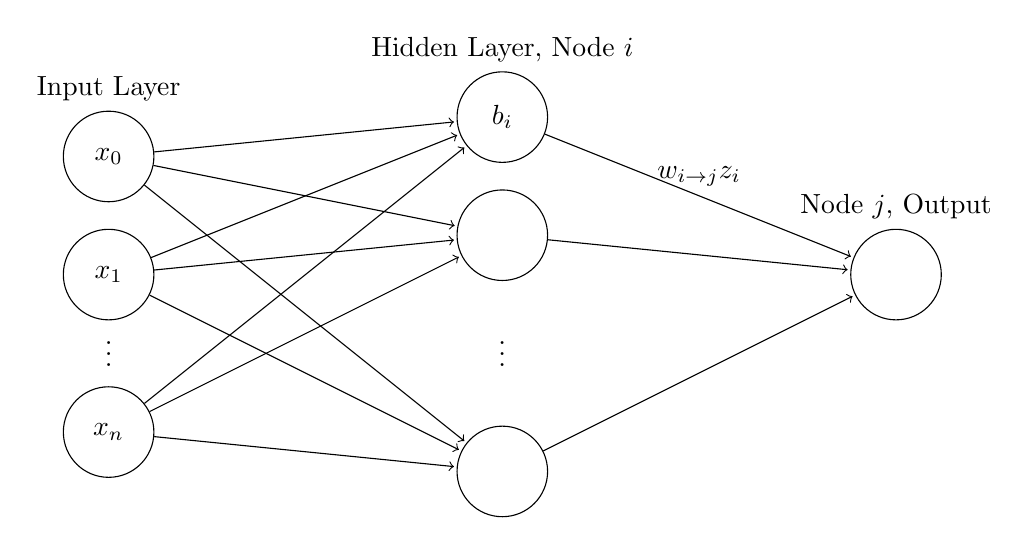
\begin{tikzpicture}[shorten >=1pt]
	\tikzstyle{unit}=[draw,shape=circle,minimum size=1.15cm]

	\node[label={Input Layer},unit](x0) at (0,3.5){$x_0$};
	\node[unit](x1) at (0,2){$x_1$};
	\node at (0,1.1){\vdots};
	\node[unit](xd) at (0,0){$x_n$};

	\node[label={Hidden Layer, Node $i$}, unit](h10) at (5,4){$b_i$};
	\node[unit](h11) at (5,2.5){};
	\node at (5,1.1){\vdots};
	\node[unit](h1m) at (5,-0.5){};

	\node[label={Node $j$, Output},unit](y2) at (10,2){};

	\draw[->] (x0) -- (h10);
	\draw[->] (x0) -- (h11);
	\draw[->] (x0) -- (h1m);
	
	\draw[->] (x1) -- (h10);
	\draw[->] (x1) -- (h11);
	\draw[->] (x1) -- (h1m);

	\draw[->] (xd) -- (h10);
	\draw[->] (xd) -- (h11);
	\draw[->] (xd) -- (h1m);

	\draw[->] (h10) -- (y2) node[midway, above] {$w_{i \rightarrow j} z_i$};

	\draw[->] (h11) -- (y2);

	\draw[->] (h1m) -- (y2);

\end{tikzpicture}
\caption[Layout of an MLP]{Layout of a Multi-Layer Perceptron\footnotemark}
\label{fig:MLP}
\end{figure}

\footnotetext{$w_{i \rightarrow j} z_i$ is the weight associated with the output
of node $i$ as the input to node $j$ multiplied by the output of node $i$, $z_i$. $b_i$ is the bias associated with node $i$.}

The resulting output ($y_i'$) is fed into a \textbf{loss function} to calculate the error for this
training example. A typical loss function for this purpose is the sum of squared errors:

\begin{equation}
\text{E}(\vec{x}, \vec{y}, \vec{w}, \vec{b})  = \sum_{i=1}^{n} (y_i - y_i')^2
\end{equation}

where $\vec{w}$ and $\vec{b}$ specify the weights and biases of the NN respectively, 
$\vec{x}$ is the set of training examples,
$\vec{y}$ is the set of training labels, $n$ is the number of training examples, and $y_i$ and $y_i'$
are the training label and output value for training example $i$, respectively.

The NN adjusts its weights and biases to minimise
loss, using \textbf{gradient descent}. This optimisation algorithm
iteratively updates these parameters using the gradients calculated from the loss function until
convergence is reached. Different variations of gradient descent used for the LSTM network
will be discussed further in \cref{sec:ImplLSTM}.

The gradients are calculated as follows:
\begin{align}
\vec{w_{t+1}} &= \vec{w_t} - \lambda \frac{\delta E(\vec{x}, \vec{y}, \vec{w}, \vec{b})}{\delta \vec{w}} \Big|_\vec{w_t}\\
\vec{b_{t+1}} &= \vec{b_t} - \lambda \frac{\delta E(\vec{x}, \vec{y}, \vec{w}, \vec{b})}{\delta \vec{b}} \Big|_\vec{b_t}
\end{align}
where $\vec{w_{t+1}}$ and $\vec{b_{t+1}}$ are the weight and bias vectors at iteration $t$, respectively.
$\lambda$ is known as the learning rate, a hyperparameter\footnote{Hyperparameters are configurable
settings for ML models that are often manually tuned for optimal performance and desired run-time.} for NNs.
The learning rate must be chosen carefully; if it is too small, the NN takes exceedingly long to reach
convergence, and if too large, the NN may never find an appropriate minimum.


The weights and biases at various nodes of the NN are updated using \textbf{backpropagation}. Backpropagation
is the method for calculating $\frac{\delta E(\vec{x}, \vec{y}, \vec{w}, \vec{b})}{\delta \vec{w}}$ and
$\frac{\delta E(\vec{x}, \vec{y}, \vec{w}, \vec{b})}{\delta \vec{b}}$ for every weight $w_{i \rightarrow j}$ and bias
$b_{i}$, as shown in \cref{fig:MLP}. These can be calculated directly. The gradient at each node in a layer is
independent when the chain rule is applied, using the calculated gradients of any nodes that take input from
node $j$. Thus, we apply backpropagation to find the gradient of each weight, starting from the output node and
working our way backwards until we reach the input feature vectors. This can be summarised into the following:

\begin{align}
\frac{\delta E(\vec{x}, \vec{y}, \vec{w}, \vec{b})}{\delta w_{i \rightarrow j}} &= z_i \sigma_j(a_j) \sum_k \delta_k w_{j \rightarrow k}\\
\intertext{\indent where}
a_j &= \sum_k w_{k \rightarrow j} z_k
\end{align}

where $k$ is any node that takes the output of node $j$, $z_i$ is the value output of node $i$,
$\sigma_j$ is the activation function for the node $j$,
and $\delta_k$ is the gradient for $w_{k \rightarrow j}$ that has already been calculated.
This formulation for calculating the weights' gradients can include the gradients for the bias, if we simply
label the bias as an extra weight, multiplied by an arbitrary $z_0 = 1$. 

\subsection{Recurrent Neural Networks}
\label{sec:introRNN}

\begin{figure}[H]
\centering
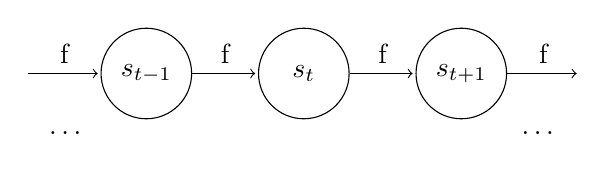
\begin{tikzpicture}[shorten >=1pt]
	\tikzstyle{unit}=[draw,shape=circle,minimum size=1.15cm]
	
	
	\node at (5,2.75){\dots};
	
	\node[unit](h0) at (6,3.5){$s_{t-1}$};
	\node[unit](h1) at (8,3.5){$s_{t}$};
	\node[unit](h2) at (10,3.5){$s_{t+1}$};
	
	\node at (11,2.75){\dots};
	
	\draw[->] (4.5,3.5) -- (h0) node[midway, above] {f};
	\draw[->] (h0) -- (h1) node[midway, above] {f};
	\draw[->] (h1) -- (h2) node[midway, above] {f};
	\draw[->] (h2) -- (11.5,3.5) node[midway, above] {f};
	
\end{tikzpicture}
\caption[States of a dynamic system]{The evolution of state in a system\footnotemark}
\label{fig:seqIn}
\end{figure}

Feed-forward networks require training examples be input into the network in full, and that
each example be independent. In the case of sequentially dependent inputs,
such as the state of a dynamic system that evolves with regards to time (\cref{fig:seqIn}), we can use
a Recurrent Neural Network (RNN).

\footnotetext{Each node represents the state at
some time $t$, which is mapped according to some underlying function f, to the state at time $t+1$.}

\begin{figure}[H]
\centering
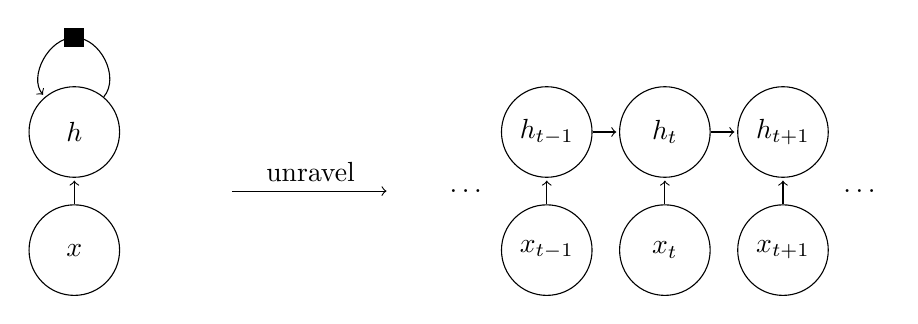
\begin{tikzpicture}[shorten >=1pt]
	\tikzstyle{unit}=[draw,shape=circle,minimum size=1.15cm]
	
	
	
	\node[unit](x) at (0,2){$x$};
	\node[unit](h) at (0,3.5){$h$};
	\draw[->] (x) -- (h);
	\draw[->] (h) to[out=50, in=0] (0,4.7) to[out=180, in=130] (h);
	\fill[black] (-0.125, 4.575) rectangle (0.125,4.825);
	
	\draw[->] (2,2.75) -- (4,2.75) node[midway, above] {unravel};
	
	\node at (5,2.75){\dots};
	
	\node[unit](h0) at (6,3.5){$h_{t-1}$};
	\node[unit](x0) at (6, 2){$x_{t-1}$};
	\draw[->] (x0) -- (h0);
	
	\node[unit](h1) at (7.5,3.5){$h_{t}$};
	\node[unit](x1) at (7.5, 2){$x_{t}$};
	\draw[->] (x1) -- (h1);

	\node[unit](h2) at (9,3.5){$h_{t+1}$};
	\node[unit](x2) at (9, 2){$x_{t+1}$};
	
	\node at (10,2.75){\dots};
	
	\draw[->] (x2) -- (h2);
	\draw[->] (h0) -- (h1);
	\draw[->] (h1) -- (h2);
	
\end{tikzpicture}
\caption[A simple RNN, in both its cyclic and unraveled form]{A simple RNN, in both its cyclic and unraveled form\footnotemark}
\label{fig:RNN}
\end{figure}

\footnotetext{(Left) The cyclic representation of an RNN. The rectangle in the cyclic arrow represents a delay of 1 time step.
(Right) The unraveled acyclic representation of the same RNN. This RNN processes information from a system at some time $t$ along
with the input passed from the network at time $t-1$, and uses this as an input for the network at time $t+1$.}

In a feed-forward NN, all values propagate
towards the output node. RNNs introduce the concept of cycles, such
that the output of a node at time $t$ may be used as an input to a node at time $t+1$. \cref{fig:RNN}
shows an example of a simple RNN. From the cyclic graph on the left, we can unravel the graph
to have an acyclic computational graph.

There are several different design patterns for RNNs, each with a different use case:
\begin{itemize}
	\item
	RNNs that produce an output at each time step and have recurrent connections between hidden units
	at different time steps
	
	\item
	RNNs that produce an output at each time step and have recurrent connections only from an output
	at a previous time step to hidden units at the next time step
	
	\item
	RNNs that take a whole sequence of inputs before producing a single output
\end{itemize}

For stock price prediction, the first design pattern is most useful. This is because
we expect our RNN to extract useful information about the state of the stock market and hold this
information within its hidden units, which may not be fully conveyed if we only
take the output.

The relevant equations regarding the hidden state and output of an RNN are as follows:

\begin{align}
\vec{h}^{(t)} &= \tanh(\vec{b}_h + \vec{W}_{hh}\vec{h}^{(t-1)} + \vec{W}_xh\vec{x}^{(t)})\\
\vec{o}^{(t)} &= \vec{b}_o + \vec{W}_{oh}\vec{h}^{(t)}
\end{align}

where $\vec{h}^{(t)}$ represents the hidden state of the RNN unit at time $t$,
and $\vec{o}^{(t)}$ represents the output of the RNN unit at time $t$. The various
$\vec{W}$s represent the weights associated with the previous 
time step's hidden value, the current input, and the current hidden state value, respectively.
The variables $\vec{b}$ represent the biases of the hidden state and the
output, respectively\footnote{For reference, the weights are matrices, thus presented in upper case,}.

A similar backpropagation algorithm to what was described in \cref{sec:introTraining} can be used
to train such an RNN: an algorithm called \textbf{backpropagation through time} (BPTT). 
This is the application of the
previous backpropagation algorithm to the unraveled computation graph of the RNN.

The key problem with the RNN is the
\textbf{vanishing/exploding gradient problem}, which
is the tendency for gradients that are propagated through many stages
to either vanish (become negligible) or explode (become disproportionately large). While the
former is only a problem when trying to model long-term dependencies, the latter can completely
disrupt the gradient optimisation algorithm. Even without unstably small gradients, the weights given to long-term dependencies are
exponentially smaller than those given to short-term dependencies due to the repeated application
of the weight of the hidden unit over many time steps.

\subsection{Long Short-Term Memory Networks}
\label{sec:introLSTM}

The LSTM is the most popular solution to the vanishing/exploding
gradient problem of vanilla RNNs. The LSTM is based on the
idea of creating paths for dependencies through time where derivatives will neither vanish
nor explode, by introducing variability to connection weights between time steps and a learned
method of forgetting the old state.

The original proposal by Hochreiter and Schmidhuber (1997) for the LSTM states that it solves the
vanishing/exploding gradient problem by ``an efficient, gradient-based algorithm for
an architecture enforcing constant
error flow through internal states of special units."\cite{Hochreiter97}
This was the inclusion of the `state' in \cref{fig:LSTMCell}, which
is preserved in the cell across time.

This design was later improved upon by Gers et al.\ (1999),
who observed that the ``LSTM fails to learn to correctly process certain
very long or continual time series that are not \textit{a priori} segmented into 
appropriate training subsequences with clearly defined beginnings and ends"\cite{Gers99}.
This is because the values of the LSTM cell state can grow without bound if the
input stream is continuous. Thus, their paper introduced the forget gate,
whose role is to learn to reset the LSTM cell's memory contents when
the information is not needed anymore.

\begin{figure}[H]
\center\textbf{LSTM Cell}
\centering
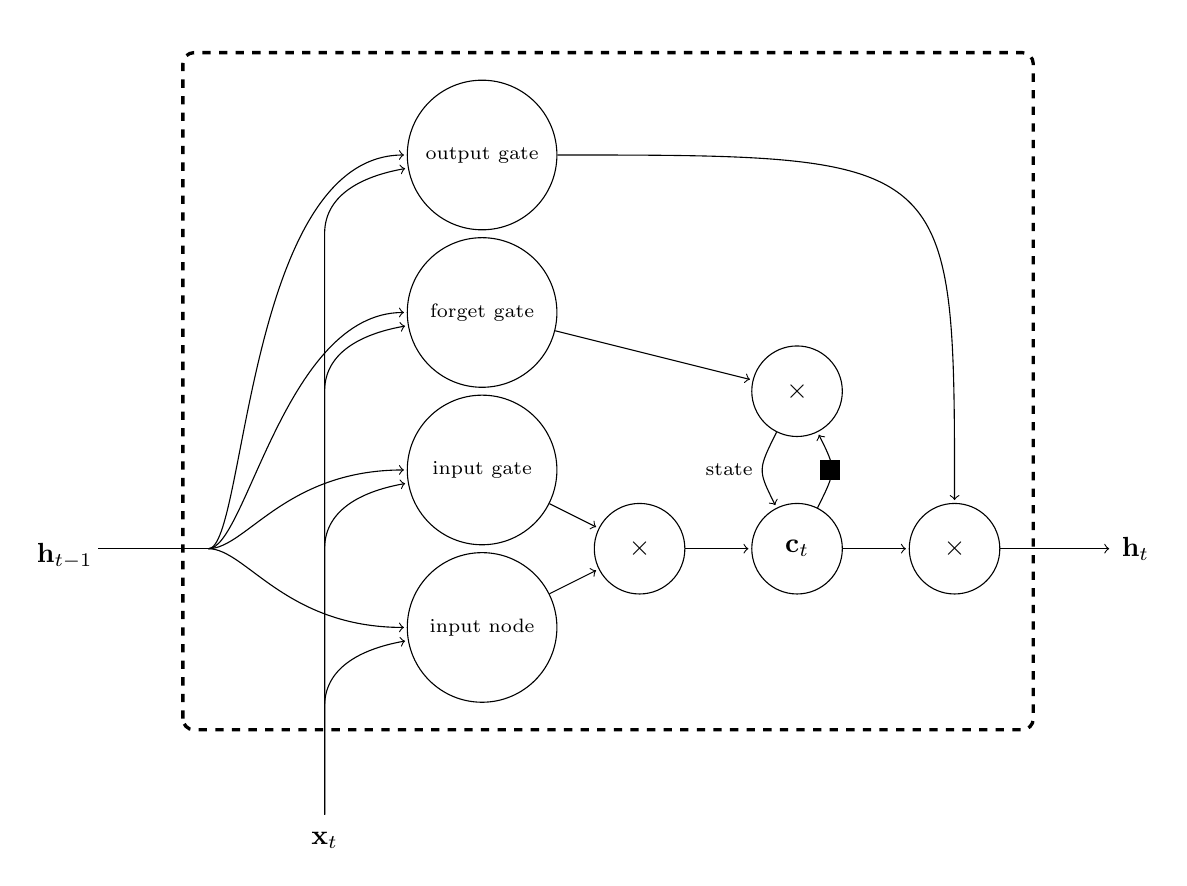
\begin{tikzpicture}[shorten >=1pt]
	\node(vspace) at (0,10){};
	
	\tikzstyle{unit}=[draw,shape=circle,minimum size=1.15cm]
	
	\tikzstyle{gate}=[draw,shape=circle,minimum size=1.9cm]
	
	\node(rec) at (1,0) {};
	\node at (1,-0.2){$\vec{x}_t$};
	\node[label={[align=center]$\vec{h}_{t-1}$}](recText) at (-2.3,3){};
	\node[minimum size=0.1pt,scale=0.1](in) at (0,3.5) {};
	\node(inHelp) at (-0.6,3.5) {};
	\node(trueIn) at (-2,3.5) {};
	
	\node[gate](input) at (3,2.5){\scriptsize{input node}};
	\node[gate](inGate) at (3,4.5){\scriptsize{input gate}};
	\node[gate](forget) at (3,6.5){\scriptsize{forget gate}};
	\node[gate](outGate) at (3,8.5){\scriptsize{output gate}};
	
	
	\node[unit](inx) at (5,3.5){$\times$};
	\node[unit](hiddenP) at (7,3.5){$\vec{c}_t$};
	
	\node[unit](hidden) at (7,5.5){$\times$};
	\node[unit](outx) at (9,3.5){$\times$};
	
	
	%\draw[->] (trueIn) to[in=180,out=180] (in) to[in=110,out=0] (0.5,2.5) to[in=180,out=-110] (input);
	%\draw[->] (trueIn) to[in=180,out=180] (in) to[in=-110,out=0] (0.5,4.5) to[in=180,out=110] (inGate);
	%\draw[->] (trueIn) to[in=180,out=180] (in) to[in=-120,out=0] (0.5,6.5) to[in=180,out=120] (forget);
	%\draw[->] (trueIn) to[in=180,out=180] (in) to[in=-130,out=0] (0.5,8.5) to[in=180,out=130] (outGate);
	
	\draw (trueIn) to[out=0, in=180] (-0.423,3.5);
	
	\draw[->] (inHelp) .. controls (in) and (0.5,2.5) .. (input);
	\draw[->] (inHelp) .. controls (in) and (0.5,4.5) .. (inGate);
	\draw[->] (inHelp) .. controls (in) and (0.5,6.5) .. (forget);
	\draw[->] (inHelp) .. controls (in) and (0,8.5) .. (outGate);
	
	\draw[->] (rec) to[out=90, in=-90] (1,1.5) to[out=90,in=190]  (input);
	\draw[->] (rec) to[out=90, in=-90] (1,3.5) to[out=90,in=190] (inGate);
	\draw[->] (rec) to[out=90, in=-90] (1,5.5) to[out=90,in=190] (forget);
	\draw[->] (rec) to[out=90, in=-90] (1,7.5) to[out=90,in=190] (outGate);
	
	\draw[->] (input) -- (inx);
	\draw[->] (inGate) -- (inx);
	\draw[->] (inx) -- (hiddenP);
	
	\draw[->] (hidden) .. controls (6.5,4.5) .. (hiddenP) node[midway, left] {\scriptsize{state}};
	\draw[->] (hiddenP) .. controls (7.5,4.5) .. (hidden);
	
	\fill[black] (7.545, 4.375) rectangle (7.295,4.625);
	
	\draw[->] (hiddenP) -- (outx);
	
	\draw[->] (forget) -- (hidden);
	\draw[->] (outGate) .. controls (9,8.5) .. (outx);
	
	\draw[->] (outx) -- (11,3.5) node[right] {$\vec{h}_t$};
	
	\draw[rounded corners, dashed, very thick] (-0.8, 1.2) rectangle (10, 9.8) {};
	
\end{tikzpicture}
\caption[Diagram of an LSTM cell]{The computational graph of an LSTM cell\footnotemark}
\label{fig:LSTMCell}
\end{figure}

\footnotetext{The black rectangle on the arrow between the looping nodes represents a delay of 1 time step.}

\cref{fig:LSTMCell} shows the computational graph of an LSTM cell at time $t$, where $\vec{x}_t$ is
the input vector at time $t$, $\vec{c}_t$ is cell activation vector at time $t$,
and $\vec{h}_t$ and $\vec{h}_{t-1}$ are the outer occurrences (and outputs) of the RNN at times $t$ and $t-1$, respectively.

The formulation for the various gates, nodes, and outputs shown are as follows:
\begin{itemize}
	\item
	Input gate
	\begin{equation}
		\vec{i}_t = \sigma(\vec{W}_{xi}\vec{x}_t + \vec{W}_{hi}\vec{h}_{t-1} + \vec{W}_{ci}\vec{c}_{t-1} + \vec{b}_i)
	\end{equation}
	
	\item
	Forget gate
	\begin{equation}
		\vec{f}_t = \sigma(\vec{W}_{xf}\vec{x}_t + \vec{W}_{hf}\vec{h}_{t-1} + \vec{W}_{cf}\vec{c}_{t-1} + \vec{b}_f)
	\end{equation}
	
	\item
	Cell activation
	\begin{equation}
		\vec{c}_t = \vec{f}_t\vec{c}_{t-1} + \vec{i}_t\tanh(\vec{W}_{xc}\vec{x}_t + \vec{W}_{hc}\vec{h}_{t-1} + \vec{b}_c)
	\end{equation}
	
	\item
	Output gate
	\begin{equation}
		\vec{o}_t = \sigma(\vec{W}_{xo}\vec{x}_t + \vec{W}_{ho}\vec{h}_{t-1} + \vec{W}_{co}\vec{c}_{t-1} + \vec{b}_o)
	\end{equation}
	
	\item
	Output
	\begin{equation}
		\vec{h}_t = \vec{o}_t\tanh(\vec{c}_t)
	\end{equation}
	
\end{itemize}
where $\sigma$ is the logistic sigmoid function, and all of the gates and the outputs are vectors
of the same size. The weight matrices ($\vec{W}$) in each gate are diagonal, so each element $m$ in the gate
vector only receives input from the respective element $m$ of the input vectors. 

\subsection{Deep LSTM Network}
\label{sec:introDeepLSTM}

Graves et al.\ (2013) showed that LSTMs provide much stronger prediction capabilities if `stacked'
in the form of hidden layers between the input and output, similar to the manner of typical deep
NNs\cite{Graves13}. We will call this a \textbf{deep LSTM network}.
The structural implication of stacking layers is that the outputs of a layer
are fed as the inputs to the next layer, and each layer is a collection of independent
LSTM cells. The advantage of this model is that it can approximate functions that are non-linear --
the more layers in the network, the more complex the possible approximation.

In this schema, the number of LSTM cells in each hidden layer is kept constant
to incorporate a direct single output-input relationship between cells of consecutive layers.
The final output $\vec{y}_t$ of the LSTM network is then a final output calculation defined by:

\begin{equation}
	\vec{y}_t = \vec{W}_{\vec{h}^Ny}\vec{H}_t^N + \vec{b}_y
\end{equation}

where $N$ is the total number of layers in the LSTM network, and $\vec{H}_t^N$ is the matrix
of the $h_t$ vectors for all LSTM cells in layer $N$.

This deep LSTM network structure is what I chose as my primary learning model
framework for stock price prediction. This framework's capacity to learn
long and short-term dependencies in data makes it suitable for a
variety of learning tasks whose inputs are sequential, such as time series prediction,
speech recognition, semantic parsing, and even composition of music\footnote{\url{http://people.idsia.ch/~juergen/blues/}}. 
Thus, it is a good candidate for tackling the learning problem of stock price prediction.

\section{Sentiment Classifiers}

\subsection{Support Vector Machines}
\label{sec:introSVM}

The theory behind Support Vector Machines in this section is adapted from
\cite{Holden18}.

\begin{figure}[H]
	\includegraphics[width=\textwidth]{SVMDataCrop.png}
	\caption[Example of the kernel trick]{Separating linearly inseparable data by introducing an additional dimension\footnotemark}
	\label{fig:SVMSep}
\end{figure}

\footnotetext{The additional dimension is $x_1x_2$. The green plane indicates the plane of separation between classes.}

Support Vector Machines (SVMs) are currently the gold standard for learning problems where
there is low availability of data. Because sentiment
labelling of the Twitter dataset was performed manually (resulting in a small sample size), the SVM is a prime candidate
for our sentiment classification problem.

SVMs tackle the problem of computing a model
for linearly inseparable data. \cref{fig:SVMSep} displays the \textbf{kernel trick}, which is the
introduction of new dimensions dependent on the original dimensions in order to increase linear separability.
This is the main idea behind SVMs.

SVMs are generally used for supervised learning, similar to most NNs. The derivation
for SVMs starts similarly to NNs -- SVMs attempt to create a hypothesis function
that maps inputs to labelled outputs, which can be generalised for unseen inputs.
The decision function starts similarly:

\begin{equation}
y = \text{sign}(\vec{wx} + b)
\end{equation}

where sign replaces the original $\sigma$.
In order to make this linear classifier non-linear, we can introduce \textbf{basis functions} $\phi_i$\cite{Holden18}:

\begin{align}
\begin{split}
	\vec{\Phi}^T(\vec{x}) &= 
	\begin{bmatrix}
	\phi_1(\vec{x})\ \phi_2(\vec{x}) \dots \phi_k(\vec{x})
	\end{bmatrix}\\
	h(\vec{x}) &= \text{sign}(\vec{w}^T\vec{\Phi}(\vec{x}) + b)
\end{split}
\end{align}

Kernels $K(\vec{x}',\vec{x})$ are selected functions that are the inner product of basis functions.
They are used to transform the decision boundary to be computable:

\begin{align}
\begin{split}
	K(\vec{x}',\vec{x}) &= \vec{\Phi}^T(\vec{x}')\vec{\Phi}(\vec{x})\\
	h(\vec{x}) &= \text{sign}(b + \vec{w}^T\vec{\Phi}(\vec{x}))\\
	&=\text{sign}(b + \sum_{i=1}^m \alpha_iy_i\vec{\Phi}^T(\vec{x}_i)\vec{\Phi}(\vec{x}))\\
	&=\text{sign}(b + \sum_{i=1}^m \alpha_iy_i K(\vec{x}_i,\vec{x}))
\end{split}
\end{align}
where $m$ is the total number of training examples, and $\vec{w} = \sum_{i=1}^m \alpha_iy_i\vec{\Phi}(\vec{x}_i)$
arises from solving
the constrained optimisation problem:\\

\noindent Minimise
\begin{equation}
\frac{1}{2}||\vec{w}||^2 + C \sum_{i=1}^m \xi_i
\end{equation}
such that
\begin{equation}
y_if(\vec{x}_i) >= 1-\xi_i\ \text{and\ } \xi_i >= 0\ \text{for\ } i = 1,...,m
\end{equation}
by solving the Lagrangian
\begin{equation}
\begin{split}
L(\vec{w}, b, \vec{\xi}, \vec{\alpha}, \vec{\lambda}) &= \frac{1}{2}||\vec{w}||^2 + C \sum_{i=1}^m \xi_i\\
&\quad - \sum_i\alpha_i(y_if(\vec{x}_i) + \xi_i - 1) - \sum_i\lambda_i\xi_i
\end{split}
\end{equation}
where minimising $\frac{1}{2}||\vec{w}||^2$ is equivalent to maximising margins, $\vec{\xi}$ is the measurement
of error(misclassification) and
$C \sum_{i=1}^m \xi_i$ is minimised for minimal error for some hyperparameter $C$\footnote{The exact methods for solving this
optimisation problem are beyond the scope of this project and will not be discussed.}.

The two most common kernel functions are the Polynomial Function
\begin{equation}
	K_{cd}(\vec{x}',\vec{x}) = (c + \vec{x}'^T\vec{x})^d
\end{equation}
where $c$ and $d$ are hyperparameters, and the Radial Basis Function (RBF)
\begin{equation}
	K_{\sigma^2}(\vec{x}',\vec{x}) = \exp(-\frac{1}{2\sigma^2}||\vec{x}'-\vec{x}||^2)
\end{equation}
where $\sigma$ is a hyperparameter. We will be using the RBF kernel for sentiment classification,
as it defines a larger function space, thus capable of modelling more non-linear functions.

\subsection{Naive Bayes}
\label{sec:introNB}

When tackling a complex learning problem, it is good practice to start with
a simple model. A Naive Bayes (NB) model is an application of
Bayes' theorem for classification based on conditional probability, 
with the `naive' assumption that the random variables
constituting features are \textbf{independent}.

The key idea of NB is to classify an example 
\begin{equation}
\vec{x} = [x_1\ x_2\ ...\ x_n]
\end{equation}
as a class 
\begin{equation}
C_k \in \{C_1, C_2, ..., C_K\}
\end{equation}
by choosing the class $C_k$ representing by
\begin{equation}
\Pr(C_k | x_1\ x_2\ ...\ x_n)
\end{equation}
which is the probability
that an example is of class $C_k$ conditioned on its features\footnote{Note that $K$ denotes the total number of possible classes.}.
By application of Bayes' theorem:
\begin{equation}
\Pr(C_k | \vec{x}) = \frac{\Pr(C_k)\Pr(\vec{x}|C_k)}{\Pr(\vec{x})}
\end{equation}
In practice, we are only concerned with the numerator, since $\Pr(\vec{x})$ is not dependent
on the class $C_k$. $\Pr(C_k)\Pr(\vec{x}|C_k)$ is equivalent to $\Pr(\vec{x}\, C_k)$, and 
since we made the assumption that each feature is independent:
\begin{align}
\begin{split}
\Pr(\vec{x}\, C_k) &= \Pr(x_1 | x_2\ ...\ x_n\ C_k)\Pr(x_2 | x_3\ ...\ x_n\ C_k)\ ...\ \Pr(x_n | C_k)\Pr(C_k)\\
&= \Pr(C_k)\prod_{i=1}^n \Pr(x_i | C_k)
\end{split}
\end{align}

Our classifier's output is then $h = C_k$ for the class satisfying

\begin{equation}
\argmax_k\quad \Pr(C_k)\prod_{i=1}^n \Pr(x_i | C_k)
\end{equation}

Where the probability $\Pr(C_k)$ is estimated by counting
the number of training examples in each class.

The types of NB classifiers, such as Gaussian NB and Multinomial NB,
differ in the assumed distributions of $\Pr(x_i | C_k)$. 

For Gaussian NB, the likelihood of a feature is assumed to be Gaussian:
\begin{equation}
	\Pr(x_i | C_k) \approx \frac{1}{\sqrt{2\pi\sigma_{C_k}^2}} \exp\bigg(-\frac{(x_i - \mu_{C_k})^2}{2\sigma_{C_k}^2}\bigg)
\end{equation}

Similarly, for Multinomial NB, the likelihood of a feature is assumed to be Multinomial. This is used
for when the features are counts of distinct events. The 
conditional probability is estimated\cite{Manning08}:
\begin{equation}
	\Pr(x_i | C_k) \approx \frac{1 + \sum_j^n x_i^j}{1 + \sum_m^n \sum_j^n x_m^j} \qquad \forall j.\ y^j=C_k
\end{equation}

An optimisation to combat decimal underflow is to instead calculate the logarithm of this conditional probability,
since $\log$ is a monotonically increasing function and no probability for any class should $= 0$.
\begin{align}
&\argmax_k\quad \Pr(C_k)\prod_{i=1}^n \Pr(x_i | C_k)\\
&=\argmax_k\quad \log\Big(\Pr(C_k)\prod_{i=1}^n \Pr(x_i | C_k)\Big)\\
&= \argmax_k\quad \log\big(\Pr(C_k)\big) + \sum_{i=1}^n \log\big(\Pr(x_i | C_k)\big)
\end{align}

\subsection{Rejected Approach}
\label{sec:prepRej}

As an initial approach to the sentiment analysis problem, \textbf{semi-supervised learning} was attempted
on a large Twitter dataset. This meant a larger dataset
was used, with only a small subset of the data being labelled. The classifier was an iterative application
of an SVM on the labelled dataset, where it would find the unlabelled examples that were clearly
separated by the decision boundary and assign the predicted label to those examples. The training process
was then re-run with the newly autonomously labelled examples in the training set, until all examples
were eventually labelled by the SVM. This process is known as \textbf{Label Spreading}.

\cref{sec:semi} gives an overview of the implementation of this model, and the reasons why it was
ultimately scrapped.

\section{Requirements Analysis}
\label{sec:introReq}
Having studied the basics of RNNs, SVMs, and
NB, I decided the project requirements. The aim is to
perform sentiment analysis on Twitter news headlines, and to combine these results with financial time-series data
to predict stock market prices with a deep LSTM network. This splits the project into two groups --
sentiment analysis and stock price prediction.

\subsection*{Sentiment Analysis}

The goal of the sentiment analysis portion is acceptable accuracy. Due to
potential difficulties presented by the small hand-labelled dataset, high
accuracy is not expected.
In terms of functional requirements, several classifiers must be
tested, and the most suitable selected for use
with the LSTM. These classifiers will be the SVM,
Multinomial NB, and Gaussian NB. 

Because of the need for Twitter data that matches both the time period and
subject matter of the financial data, I will build a data scraping and processing
system to gather my dataset. I will also be experimenting
with several feature extraction methods from the Twitter dataset, namely
\texttt{doc2Vec}\cite{Le14} and Bag of Words.


\subsection*{Stock Price Prediction}

The goal of the project is to predict stock
prices more accurately on the test dataset than a random agent. This accuracy
measurement takes into account the mean squared error (MSE)\footnote{MSE
is calculated $\frac{1}{n} \sum_{i=1}^n (Y_i - \hat{Y}_i)^2$, for dataset size $n$,
targets $Y$, and predictions $\hat{Y}$.} of the predictions
and the prediction's directional accuracy\footnote{The percentage of samples for which the model correctly predicted a rise 
or fall.}. The functional requirements for the price prediction
section are that the sentiment classification output
must combine with the financial data, a feature extractor for financial
indicators must be built, and the LSTM must function properly, with
well-tuned hyperparameters.

A summary of the requirements for this project is shown in \Cref{table:req}.

\begin{table}[H]
\centering
\begin{tabular}{p{8cm} lll}
\toprule
\textbf{Requirement}                                                                               & \textbf{Priority} & \textbf{Risk} & \textbf{Difficulty} \\ \midrule
Multinomial Naive Bayes                                                                                     & Medium            & Medium        & Medium              \\ [0.5ex]
Gaussian Naive Bayes                                                                                        & Medium            & Medium        & Medium              \\ [0.5ex]
Support Vector Machine                                                                                                & High              & Medium        & Low                 \\ [0.5ex]
Twitter data processing                                                                            & High              & Medium        & Medium              \\ [0.5ex]
\begin{tabular}[c]{@{}l@{}}Compare and evaluate Twitter feature \\[-0.5ex] extraction methods\end{tabular} & Low               & Low           & Medium              \\ [2ex]
\begin{tabular}[c]{@{}l@{}}Compare and evaluate sentiment \\[-0.5ex] analysis models\end{tabular}          & High              & Low           & Medium              \\ [2ex]
\begin{tabular}[c]{@{}l@{}}Combine sentiment classifier output\\[-0.5ex] and financial data\end{tabular}   & High              & Medium        & Medium              \\ [2ex]
Feature extractor for financial data                                                               & Medium            & Low           & Medium              \\ [0.5ex]
Long Short-Term Memory Network                                                                                               & High              & High          & High                \\ [0.5ex]
Hyperparameter tuning                                                                              & Medium            & Low           & Medium              \\ [0.5ex] \bottomrule
\end{tabular}
\caption{Goals of the project}
\label{table:req}
\end{table}


\section{Choice of Tools}
\label{sec:introTool}

\subsection{Programming Language}

For ML projects, it is standard to use \texttt{Python}
because of its support for ML libraries (such as Tensorflow, Keras, Theano), its
ease of use, and relaxed type system. Though the language is not as
fast as other languages such as \texttt{Java} and \texttt{C++}, many of its
powerful libraries use \texttt{CPython}, a reference implementation
and interpreter of \texttt{Python} in \texttt{C}.
This allows libraries to exploit the performance of \texttt{C} while maintaining
the benefits of \texttt{Python}. I chose \texttt{Python} as the
language for my project, while also using \texttt{MATLAB} for some trivial
plotting and mathematical tasks.

\subsection{Libraries}
\label{sec:introLib}

The main third party libraries used are shown in \Cref{table:libs}. \texttt{Tensorflow}\footnote{\url{https://www.tensorflow.org/}}
and \texttt{Scikit-learn}\footnote{\url{http://scikit-learn.org/}} are
of particular importance. Both libraries are well-documented and widely used in industry, with the 
latter often used for prototyping. \texttt{GetOldTweets}\footnote{\url{https://github.com/Jefferson-Henrique/GetOldTweets-python}}
is not an official library, but an open-source
project for scraping Twitter searches.

\begin{table}[H]
\centering
\begin{tabular}{llll}
\toprule
\textbf{Library}                        & \textbf{Version} & \textbf{Use} & \textbf{License} \\ \midrule
Tensorflow                             & 1.5.0            & Building LSTM        & Apache 2.0 License              \\ [0.5ex]
Scikit-learn                           & 0.19.0           & Using SVM        & BSD-new License              \\ [0.5ex]
Numpy                                  & 1.14.0           & Efficient array manipulation        & BSD-new License              \\ [0.5ex]
Scipy                                  & 0.19.1           & Probability functions for NB        & BSD-new License              \\ [0.5ex]
Pandas                                 & 0.20.3           & Data manipulation        & BSD-new License              \\ [0.5ex]
Gensim								   & 2.3.0			  &	\texttt{Doc2vec} feature extraction			& GNU LGPLv2.1 license\\ [0.5ex]
Matplotlib							   & 2.0.2			  & Graph plotting 				& Matplotlib License	\\ [0.5ex]
GetOldTweets                           & Unknown          & Twitter web scraping        & MIT License              \\ [0.5ex] \bottomrule
\end{tabular}
\caption{Main libraries used in this project}
\label{table:libs}
\end{table}

\subsection{Development and Testing}

Development was carried out on my personal laptop, which runs Windows 10. Because of its relatively 
powerful graphics card (Nvidia GTX 1060), it was also capable of training and testing the LSTM
models.

For revision control, I used \texttt{git}, the revision control system
that is almost ubiquitous in industry. I created and synchronised repositories on
GitHub\footnote{\url{https://github.com}, a free and popular \texttt{git} repository hosting service.}
for both my project and the dissertation write-up. This was used for
tracking progress and as a back-up tool. 


\section{Starting Point}
\label{sec:introStart}

The Computer Science Tripos has several courses that proved useful for my project.
These are outlined in \Cref{table:courses}. In particular, Machine Learning and
Bayesian Inference provided me with the base knowledge required for understanding
SVMs, NB, and NNs -- however, personal study was required to
learn about RNNs, LSTMs, and hyperparameter tuning techniques.

My \texttt{Python} knowledge prior to this project was intermediate, having used it
as a minor part of a prior internship. I had no experience with \texttt{Tensorflow}
or other DL libraries. This meant I had to learn the design concepts
behind Tensorflow, which is to construct operations for NNs as
computational graphs operating on tensors. 

\begin{table}[H]
\centering
\begin{tabular}{p{8cm} l}
\toprule
\textbf{Course}                              & \textbf{Application} \\ \midrule
Machine Learning and Bayesian Inference      &  NNs, SVM                    \\
Natural Language Processing                  &  Twitter feature extraction                    \\
LaTeX and MATLAB                             &  Plotting       \\
Mathematical Methods for CS    &  Understanding probability functions            \\
Software Engineering                         &  Iterative development model                    \\\bottomrule
\end{tabular}
\caption{Tripos courses applicable to this project}
\label{table:courses}
\end{table}

\section{Software Engineering and Approach}
\label{sec:introImpl}

It is imperative to plan stages of
development and to compartmentalise the project. As outlined in \cref{sec:introReq},
the project was split into two sections: sentiment analysis and stock price prediction. A
schematic of the project's components are show in \cref{fig:overview}.

\begin{figure}[H]
\centering
\vspace{10pt}
\includegraphics[width=\textwidth]{Proj_Overview.png}
\caption{Overview of project components}
\label{fig:overview}
\end{figure}

The \textbf{Iterative and Incremental Development Model} was adopted for this project.
The idea was to first build a `walking skeleton' -- a runnable end-to-end system that
has all essential components of the final product, though components
may be placeholders\cite{Cockburn04}. These components can be properly
implemented at a later date, with the project's architecture already in place.
These components were then iteratively tuned and improved.

The list of components to complete were as follows, ranked by implementation order:

\begin{enumerate}
\item
Collect Twitter and financial data

\item
Manually label Twitter dataset

\item
Implement sentiment feature extractors

\item
Build Gaussian and Multinomial NB

\item
Build SVM

\item
Evaluate and pick the most accurate classifier

\item
Implement financial feature extractor

\item
Build LSTM
\end{enumerate}
The components described in steps 4-9 were then iteratively refined after initial completion.


\section{Summary}
\label{sec:prepSumm}

In this chapter, I have discussed the relevant theory that was learned and the planning
that occurred before implementation was started. I gave an introduction to the concepts
behind the ML models I will be implementing, and outlined the goals and
key development strategies. I also gave an overview of the tools and libraries I
will be using.

The next chapter will detail the implementation of the project, showing how the goals and
plans outlined in this chapter were achieved.

\chapter{Implementation}
\label{sec:imp}

This chapter details the implementation of the project, and how the goals and
design principles outlined in the previous chapter were accomplished. I will
present the sentiment analysis portion first, before moving into price
prediction. This was the order in which I implemented the project and provides a logical flow between the components.

\section{Sentiment Analysis}
\label{sec:impSenti}
This section first gives an overview of the rejected approach to the
learning problem. The rest of the section is discussed in the order of data flowing 
through the system --
we discuss the collection of data, before
moving onto feature extraction, and finally the different sentiment classifiers.

\subsection{Rejected Approach}
\label{sec:impFailed}

\subsubsection{Semi-Supervised Learning}
\label{sec:semi}
My first experiment with the sentiment analysis problem was to
acquire as much relevant data as possible and manually label a small subset
for a semi-supervised learning model. The reasons behind this decision
were the abundance of official Twitter accounts of large news
agencies, and that there may be a sufficient number of samples for a
semi-supervised DL model (such as a \textbf{Hybrid Deep Belief Network}\cite{Zhou14}).

My approach to examining potential solutions to a learning problem is to first
use a simple model to gain insight on whether the problem can feasibly
be solved. I used the \texttt{Scikit-learn} library's semi-supervised learning 
implementation to test semi-supervised learning
for this dataset. This module uses the label spreading method mentioned in
\cref{sec:prepRej}, combined with a standard SVM. An example of this technique is shown in \cref{fig:ls},
where the unlabelled samples furthest from the decision boundary are automatically labelled after each step.

\begin{figure}[H]
\centering
\vspace{10pt}
\includegraphics[width=\textwidth]{LabelSpreading.png}
\caption{Example of 3-step label spreading}
\label{fig:ls}
\end{figure}

After manually labelling 2000 tweets, out of
approximately 500,000 tweets, I separated the labelled dataset into an 80:20 split for train:test,
a standard ratio for partitioning data. The labelled 80\% training set was combined
with the unlabelled dataset and used to train the semi-supervised SVM. The
trained model was evaluated on the separated labelled test dataset.

The results gave little confidence in moving forward with this technique, as the accuracy 
for sentiment classification was 54\%. Considering the output is
fed into the LSTM network, it is imperative that the output be mostly correct
to ensure that inputs are kept as noise-free as possible. Thus, I decided to
pursue a supervised learning approach to the problem.

\subsection{Data}
\label{sec:impSentiData}

After experimenting with semi-supervised learning, I realised
it may be more effective to be selective about the data I was collecting. This ensures
the dataset was small enough to manually label and enforces that only relevant 
information to the price prediction model should be used.

I settled on using tweets from the official Reuters Twitter account\footnote{\url{https://twitter.com/Reuters}}.
From the semi-supervised dataset, I realised that there was much redundancy
when sampling from many accounts, since important news stories are broadcasted by most agencies.
I chose Reuters because it is a leading provider of financial news, and
news regarding specific companies were usually labelled with the corresponding ticker symbol\footnote{A ticker symbol is the identifier given to a company on
a stock exchange.}. To account for irregularities,
I also searched for mentions of the company's name in each tweet. This gathered missed data from lack of mention of the company's ticker, but also introduced
irrelevant news samples, such as Tweets mentioning the Amazon rainforest. An example of a Tweet from
this dataset is shown in \Cref{fig:reutersMSFT}.

\begin{figure}[H]
\centering
\vspace{10pt}
\includegraphics[width=\textwidth]{ReutersTweetMSFT.png}
\caption{A positive Tweet about Microsoft from the dataset}
\label{fig:reutersMSFT}
\end{figure}


Since our Twitter dataset must coincide with the financial dataset, the train:test split
for the Twitter dataset was set to match the train:test split of the financial
dataset, according to date. This means the date of the financial data at the
train:test boundary was used as the date for the train:test boundary for the Twitter
dataset.

\subsubsection{Initial Approaches}
My first approach to acquiring the Twitter dataset was to find labelled datasets from other studies
conducted regarding Twitter sentiment analysis on financial data. After failing to find any that 
were sufficiently related to my project, I moved to collect data through Twitter's official web API.
After discovering that API calls for retrieving tweets older than a week were locked
behind a paywall\footnote{\url{https://developer.twitter.com/en/docs/tweets/search/overview}}, I decided to find a way around this issue.

\subsubsection{Web Scraping}
\label{sec:impCrawl}

The limitation on historical tweet retrieval prevented me from acquiring enough data to match a financial dataset,
which needed to be suitably large for DL.
As mentioned in \cref{sec:introLib}, I used the \texttt{GetOldTweets} library for web scraping the relevant Twitter page.

This library generates a search query URL, which specifies the username, time frame, language,
search query, and maximum number of returned tweets. An HTTP GET request is sent to the search URL,
and the response of the search results in returned. This contains a page
worth of results, and the process is repeated until all results are gathered. The responses are then parsed and
converted to Tweet objects and returned from the original function call. A simplified UML diagram for this
Tweet class is shown in \Cref{fig:UMLTweet}. Note that, since this class is used as a
data structure, all variables are public. This removes the need for \texttt{getter} and \texttt{setter} methods.

\begin{figure}[H]
\centering
\begin{tikzpicture}
	\umlclass{Tweet Class}{
		+id : \texttt{String}\\
		+link : \texttt{String}\\
		+username : \texttt{String}\\
		+text : \texttt{String}\\
		+date : \texttt{Datetime.Datetime}\\
	}{}
\end{tikzpicture}
\caption{Simplified UML class diagram for Tweet}
\label{fig:UMLTweet}
\end{figure}

As shown in the earlier \Cref{fig:reutersMSFT}, some Tweets contain
a URL. These URLs are irrelevant for sentiment analysis, and were filtered using
regular expressions.

\subsubsection{Labelling}
\label{sec:impLabel}

Because of the need for manual labelling, criteria for labels were established
to minimise human bias. However, sentiment is inherently
subjective, raising a small but unavoidable issue with manually labelled datasets.

Nevertheless, the criteria for labelling are as follows:

\begin{itemize}
\item
If the news is irrelevant (e.g.\ mentioning the Amazon rainforest rather than the company),
or if the news does not seem positive or negative, or it contains mixed sentiment, the Tweet is labelled $0$

\item
If the news is deemed to have possible positive effects on a company's financials, the Tweet is labelled $1$

\item
If the news is deemed to have possible negative effects on a company's financials, the Tweet is labelled $-1$
\end{itemize}

\subsection{Features}
\label{sec:impSentiFeat}
I used two feature extraction systems for the Twitter dataset. The first is
Bag of Words. This is the vector representation for word occurrence counts --
we first build a vocabulary of words by parsing through the training dataset to find a list of all unique words,
assigning an index to each unique word. We then build feature vectors of $m$ length, where $m$ is the
total number of unique words in the dataset. For every word in the training example, we
increment the value at the corresponding index for the word in the feature vector. This is
a tally for each unique word in the example, with zeros where the
corresponding word does not appear in the example. A visual example is shown in \cref{fig:bow}.

\begin{figure}[H]
\centering
\vspace{10pt}
\includegraphics[width=\textwidth]{BoW.png}
\caption{Diagram of Bag of Words vocabulary and vector representation}
\label{fig:bow}
\end{figure}


For cases where unique words appear in the test/validation
dataset but not in the training set, we can include an extra dimension in the feature
vector for `other'. However, since the training data does not include any examples featuring
this word, the model will either not have trained to include it in its decision boundary, or unexpected
behaviour may occur. Thus, it is better practice to omit new unique words when extracting features
from the test/validation sets.

The current state-of-the-art feature representation method for text is \texttt{doc2vec}\cite{Le14},
which is a continuation of \texttt{word2vec}\cite{Mikolov13}. \texttt{Word2vec} is an unsupervised method
for vector representation of words. The idea is that words of similar meaning are closer by Euclidian distance in the feature vector space than
words that are not related. \cref{fig:word2vec} also shows that logical vector relations 
also follow from this property, in that the feature vector for a word can be deconstructed
combinations of feature vectors that are logically computed in the realm of semantic relations.
The example in the figure is that $\vec{King}$ is to $\vec{Queen}$ what $\vec{Man}$ is to $\vec{Woman}$,
and $\vec{King} - \vec{Man} + \vec{Woman} = \vec{Queen}$. This shows that
logical combinations of words' semantic meanings are directly translated to addition and subtraction in
the feature vector space.

\begin{figure}[H]
\centering
\vspace{10pt}
\includegraphics[width=\textwidth]{word2vec.png}
\caption{Simplified \texttt{word2vec} representation of words}
\label{fig:word2vec}
\end{figure}

This feature representation is generated through an unsupervised feedforward NN. There
are two models for \texttt{word2vec} -- \textbf{continuous bag of words} (CBOW) and \textbf{skip-gram}.
CBOW is a Bag of Words method that uses the context of a word to predict the given word.
CBOW uses one-hot-encoding vectors
for words within a given window around the selected word in a sentence. These vectors are averaged,
and fed through a NN with a single hidden layer 
and output layer to predict the selected word. The output layer is a \textbf{softmax}
layer, a generalised version of the logistic sigmoid function explained in \cref{sec:prepNeurons},
applying the sigmoid function to every element of a vector.
The weights for the hidden layer, after training, are translated into the feature extractor.
The skip-gram model works in the opposite
direction -- given a word, it predicts the
context of the word (average of the words within the specified window around the selected word).
The skip-gram model is much slower to train, but is more accurate for infrequent words.

The \texttt{doc2vec} method abstracts the \texttt{word2vec} methods to a vector representation
for a whole document. The model predicts the word within a paragraph given its context, as well
as a paragraph ID, represented in a one-hot-encoding vector. The context and paragraph ID can
either be averaged together, such as in CBOW in \texttt{word2vec}, or concatenated. Averaging
results in a model that disregards word order, but requires substantially fewer
examples to train. We will be using the averaging method, as our dataset is not sufficiently
large for concatenation. The architecture for single hidden layer and softmax output layer are
the same as for the \texttt{word2vec} model, meaning we use the hidden layer's weights as our
feature extractor after training the \texttt{doc2vec} model.

\begin{figure}[H]
\centering
\begin{tikzpicture}
	\umlclass{Doc2vec Class}{
		+documents : \texttt{int[][][]}\\
		+CBOW : \texttt{int}\\
		+vectorSize : \texttt{int}\\
		+windowSize : \texttt{int}\\
		+init\_learningRate : \texttt{int}\\
		+epochs : \texttt{int}\\
		+totalExamples : \texttt{int}
	}{
		+\_\_init\_\_(documents : \texttt{int[][][]}, CBOW : \texttt{int}, vectorSize : \texttt{int},\\
		\qquad windowSize : \texttt{int}, init\_learningRate : \texttt{int}) : \texttt{void}\\
		+buildVocab(documents : \texttt{int[][][]}) : \texttt{void}\\
		+train(documents : \texttt{int[][][]}, totalExamples : \texttt{int}, epochs : \texttt{int}) : \texttt{void}\\
		+inferVector(documents : \texttt{int[][][]}) : \texttt{int[][]}
	}
\end{tikzpicture}
\caption{Simplified UML class diagram for \texttt{gensim}'s \texttt{doc2vec}}
\label{fig:UMLd2v}
\end{figure}

I used the \texttt{gensim} library's implementation of \texttt{doc2vec} as a feature extractor.
The simplified UML diagram for this implementation is shown in \Cref{fig:UMLd2v}. The key
variables and hyperparameters are shown below. The values chosen for these hyperparameters were the recommended values
found in literature.

\begin{itemize}
\item
Documents -- An array of \texttt{named tuples}.
Each \texttt{named tuple} contains the Tweet's text split into an array of words
and a unique tag for every document

\item
BOW -- A parameter specifying whether to use the averaging implementation (1) or the
concatenating implementation (0), set to 1

\item
VectorSize -- Desired dimensionality of the extracted vector, set to 100

\item
WindowSize -- Size of window from which context is taken, set to 10

\item
Init\_learningRate -- The initial learning rate of the NN, set to 0.1

\item
Epochs -- The number of steps for which the NN trains, set to 32 and 64, as hyperparameters
in cross-validated grid-search (discussed in \cref{sec:classSelect})

\item
TotalExamples -- The total number of Tweets
\end{itemize}

\subsection{Naive Bayes}
\label{sec:impNB}
This section will explain the implementation of each NB classifier.

The versions of the NB classifier were chosen because they are
well-suited to our two feature extraction methods. Gaussian NB, which accepts
feature vectors of real values (with the assumption that the features have a Gaussian distribution),
is the most fitting NB classifier for \texttt{doc2vec}. Multinomial NB,
which accepts feature vectors where each feature is a count of an event (with the assumption
that the counts have a Multinomial distribution), is perfect for Bag of Words.

\subsubsection{Gaussian Naive Bayes}
\label{sec:impGNB}

\begin{figure}[H]
\centering
\begin{tikzpicture}
	\umlclass{Gaussian Naive Bayes Class}{
		+summaries : \texttt{int[][]}\\
		+probabilities : \texttt{int[]}
	}{
		+train(trainSet : \texttt{int[][]}, trainLabels : \texttt{int[]}) : \texttt{void}\\
		+test(testSet : \texttt{int[][]}, testLabels: \texttt{int[]}) : \texttt{int}\\
		+predict(testSample : \texttt{int[]}) : \texttt{int}\\
		\\
		+summarise(trainSet : \texttt{int[][]}) : \texttt{int[][]}\\
		+calcLogClassProbabilities(summaries : \texttt{int[]}, sample : \texttt{int[]}) : \texttt{int[]}
	}
\end{tikzpicture}
\caption{UML class diagram for Gaussian Naive Bayes implementation}
\label{fig:UMLGNB}
\end{figure}

The Gaussian NB classifier was implemented with two main functions that affect training
and testing -- \texttt{summarise} and \texttt{calcLogClassProbabilities}, as shown in \Cref{fig:UMLGNB}.
The summaries that are calculated contain the means and standard deviations of each attribute, for each
class value. This is given to \texttt{calcLogClassProbabilities} to calculate the probability
that the sample belongs to each class, based on the assumption that each feature is normally distributed.

Upon implementing the class, I realised that \texttt{Scikit-learn}'s implementation
of Gaussian NB was much faster than my implementation, with the same results. This is probably
due to vector optimisations in the library's implementation. I therefore decided
to use the library's Gaussian NB classifier for testing, which had similar \texttt{train}, \texttt{test}, and \texttt{predict}
functions, called \texttt{fit}, \texttt{score}, and \texttt{predict}.

\subsubsection{Multinomial Naive Bayes}
\label{sec:impMNB}

The Multinomial NB classifier was implemented similarly to the Gaussian NB classifier, with similar
main functions \texttt{summarise} and \texttt{calcLogClassProbabilities}. Again, the same model
from \texttt{Scikit-learn} was much faster, and was selected for testing.
The main interfacing functions were \texttt{fit}, \texttt{score}, and \texttt{predict}.

The code for the implementation of Multinomial NB can be found in \Cref{appendix:NB}.

\subsection{Support Vector Machine}
\label{sec:impSVM}

The implementation of an SVM is beyond the scope of this project.
I used the \texttt{Scikit-learn} library's Multi-Class SVM implementation,
since we have three classes: $-1$, $0$, and $1$.

The Multi-Class SVM implementation is an extension of a regular SVM --
this object trains $\frac{n (n-1)}{2}$ SVM classifiers, where $n$ is the number
of classes. Each individual classifier is trained to differentiate a combination
of two classes. The Multi-Class SVM selects the most likely class for a test example 
given the predictions and decision boundaries for each individual classifier.

The main interfacing functions from this class are again \texttt{fit}, \texttt{score},
and \texttt{predict}.

\subsection{Classifier Selection}
\label{sec:classSelect}
The four classifiers (BoW Multinomial Naive Bayes, \texttt{doc2vec} Gaussian Naive Bayes, BoW SVM, \texttt{doc2vec} SVM)
were compared for selection. The SVM's hyperparameters, $C$ and $\gamma$, and \texttt{doc2vec}'s epochs were
optimised using 10-fold
cross-validated grid search.

\textbf{Cross-validation} is a method for partitioning data so that experiments can be carried out
on the learning model without using the test dataset. Cross-validation partitions the
training data into a training and validation set, usually with the same ratio as
train:test. The hyperparameters that perform best on the
validation set is selected for use in the overall training.

\textbf{K-fold cross-validation} is the method of using cross-validation $k$ times across
the training dataset. Unique examples in the validation set 
are chosen for every fold of the process, and every example in the training set is used 
in a validation set at some point during
the k-fold process. The estimate for performance is then:

\begin{equation}
\frac{1}{k} \sum_{i = 1}^k \hat{E}_{S^{(i)}} (L_{S^{(-i)}p})
\end{equation}

where $S^{(-i)}$ denotes the set obtained from training set $S$ by removing
validation set $S^{(i)}$, $L_{S^{(-i)}p}$ denotes a learning algorithm
$L$ that has been trained on set $S^{(-i)}$ using hyperparameters $p$,
and $\hat{E}_{S^{(i)}} (h)$ denotes an error measurement
for learning algorithm $h$\footnote{Adapted from \cite{Holden18}.}.

For our SVMs, since they only have two hyperparameters $C$ and $\gamma$,
it is possible to perform a \textbf{grid search} on the possible viable values for each
hyperparameter. Grid search is an exhaustive search for every combination of values,
which is the common method of hyperparameter optimisation for SVMs.

The viable values for the SVMs that were selected are shown in \Cref{table:SVMhyper}.

\begin{table}[H]
\centering
\vspace{10pt}
\setlength{\tabcolsep}{3cm}
\begin{tabular}{c c}
\toprule
\multicolumn{2}{c}{\textbf{Values used for k-fold cross validation}}                               \bigstrut\\
\midrule
$C$                                                                & $\gamma$   \bigstrut\\
\midrule
0.1                                                                  & 0.01                        \bigstrut\\
0.5                                                                  & 0.05                        \bigstrut\\ 
1                                                                    & 0.1                         \bigstrut\\ 
5                                                                    & 0.5                         \bigstrut\\
10                                                                   & 1                           \bigstrut\\
50                                                                   & 5                           \bigstrut\\
100                                                                  & 10                          \bigstrut\\ \bottomrule
\end{tabular}
\caption{Hyperparameter values grid-searched for SVM classifiers}
\label{table:SVMhyper}
\end{table}

After cross-validation, the best SVMs were trained on the full training set, 
along with the NB classifiers (which have no hyperparameters).
The best-performing classifer on the test set (Bag of Words SVM), based on accuracy of predictions,
was selected for price prediction.

\section{Price Prediction}
\label{sec:impFin}
This section will detail the implementation of price prediction. 
We will discuss the decisions behind data selection,
the chosen technical financial features, and the implementation
of the LSTM network.

\subsection{Data}
\label{sec:impFinData}

Because of the need for manual labelling of the Twitter dataset, as mentioned in \cref{sec:impFailed} and 
\cref{sec:impSentiData}, a financial dataset with specific requirements was chosen:

\begin{itemize}
\item
The dataset must not span too large a time period, to ensure the corresponding Twitter dataset is not too large to label

\item
The dataset must not include too many stocks, to ensure the corresponding Twitter dataset is not too large to label

\item
The dataset must include enough samples, to ensure the LSTM network has sufficient data for training

\item
The dataset must be composed of relevant stocks whose companies regularly receive media attention

\item
The dataset preferably includes a representative group of stocks for an industry or the global economy

\end{itemize}

The resulting dataset comprises of a 6-month period of data for the five highest market cap\footnote{Market cap
is the total market value of a company's shares.} stocks on the
NASDAQ exchange: Apple, Amazon, Alphabet\footnotemark ($\times2$), and Microsoft. The stock prices for
were sampled at 20 minute intervals. The total number of Tweets
in the dataset was 2740, while the number of samples in the financial
dataset was around 11000. This was considered acceptable, given the requirements.

\footnotetext{Alphabet is listed twice on the NASDAQ exchange, as GOOGL and GOOG. These are two separate stocks: GOOGL
holders have voting rights while GOOG holders do not.}

\subsection{Features}
\label{sec:impFinFeat}

Features for the financial data were based on technical indicators. Technical analysis
of a stock relies on numerical analysis of a stock's price or volume, while fundamental
analysis relies on gauging a company's intrinsic value. 

Technical indicators are better suited for Ml.
Often used to predict short-term movements in a stock's price, they lack a need for context,
background knowledge, and intuition, making them an easy input for Ml.
These indicators, along with the current stock
price and the most recent sentiment analysis result, are fed into the LSTM network in order
to predict stock prices.

\begin{table}[H]
\centering
\vspace{10pt}
\setlength{\tabcolsep}{0.3cm}
\begin{tabular}{p{5cm} p{9.5cm}}
\toprule
\textbf{Feature}          					& \textbf{Description}  \bigstrut\\ \midrule
Current price								& Current price, used as reference for prediction \bigstrut \\\midrule
Williams percentage range (Williams \%R)	& Measures overbuying and overselling, used with an interval to find highest and lowest prices during time frame  \bigstrut \\\midrule
Rate of change (RoC)						& Ratio of change from previous price  \bigstrut \\\midrule
Momentum									& Change of price within an interval  \bigstrut \\ \midrule
Relative strength index (RSI)				& Compares magnitude of recent gains and losses to measure speed and change of price movements  \bigstrut\\ \midrule
Triple exponential moving average (TEMA) 	& Smooth price fluctuations and filter out volatility  \bigstrut\\ \bottomrule

\end{tabular}
\caption{Financial technical indicators used as features}
\label{table:fintech}
\end{table}

\Cref{table:fintech} shows the technical indicators that were used. These indicators were selected for their
simplicity and balanced coverage of relevant factors. The mathematical formulations for the 
indicators are as follows:

\begin{equation}
\text{Williams \%R} = \frac{\text{highest price} - \text{current price}}{\text{highest price} - \text{lowest price}}
\end{equation}

\begin{equation}
\text{RoC} = \frac{\text{current price}}{\text{previous price}} - 1
\end{equation}

\begin{equation}
\text{Momentum} = \text{current price} - \text{price at previous interval}
\end{equation}

\begin{equation*}
\text{RSI} = \frac{100 \times \text{average}(\text{upgain})}{\text{average}(\text{upgain}) + \text{average}(\text{downloss})}
\end{equation*}
where
\begin{equation}
\text{upgain} = \text{price} - \text{previous price} \quad \text{when} \quad \text{price} > \text{previous price}
\end{equation}
and
\begin{equation*}
\text{downloss} = \text{previous price} - \text{price} \quad \text{when} \quad \text{price} < \text{previous price}
\end{equation*}

\begin{equation}
\text{TEMA} = 3 \times \text{EMA} - 3 \times \text{EMA}(\text{EMA}) + \text{EMA}(\text{EMA}(\text{EMA}))
\end{equation}
where EMA is the Exponential Moving Average\footnote{EMA is calculated for some series $S_t$ -- $\text{EMA}(S_t) = \alpha\text{value}_t + (1-\alpha)S_t$.}.

These financial features were combined with the sentiment classifier's output. Each sample for 
the sentiment classifier was matched with the most recent subsequent timestamp
in the financial dataset. The pseudo-code for the combination is shown
in \Cref{alg:combine}. The sentimentFeatures include both the train
and test samples, as do financialFeatures. 
Note that because we have set the train:test ratio for the Twitter dataset
and the financial dataset to match based on dates (explained in \cref{sec:impSentiData}),
the separation of train and test data is upheld.
Also note irrelevant or inconsequential Tweets, which have a label of $0$,
are effectively discarded in this function.

\begin{algorithm}[H]
\caption{Combining sentiment and financial features}\label{alg:combine}
\begin{algorithmic}
\Function{combineFeatures}{financialFeatures, sentimentFeatures}
	\Assert{sorted(financialFeatures[dates])}
	\Assert{sorted(sentimentFeatures[dates])}
	\item[]
	\LeftComment{Set return array to financialFeatures array with extra empty element}
	\item[]
	\State returnFeatures = [finFeat.append[] for finFeat in financialFeatures]
	\State lastFinIndex = 0
	\For{sentiFeat in sentimentFeatures}
		\For{i = lastFinIndex; i $<$ length(financialFeatures); i++}
			\If{financialFeatures[i].date $>$ sentiFeat.date}
				\item[]
				\LeftComment{Set the last element in returnFeatures array to accumulate}
				\LeftComment{sentiment analysis feature}
				\item[]
				\State returnFeatures[i][-1] += sentiFeat
				\Break
			\EndIf
		\EndFor
	\EndFor
	\State \Return returnFeatures
\EndFunction
\end{algorithmic}
\end{algorithm}

Note that only sentiment classification for news pertinent to the company was fed into its
prediction model. After the Twitter dataset is classified, it is
separated into individual datasets based on mention of companies before being
combined with their respective financial datasets.

\subsection{Long Short-Term Memory}
\label{sec:ImplLSTM}

This section describes the implementation of the deep LSTM network.
We will discuss its architecture, the representation
of the network as a \texttt{Tensorflow} graph, and an overview of the LSTM
network class.

We will then discuss the optimisations to the network, which are initialisation,
the weight optimiser algorithm, early stopping, and hyperparameters.

\subsubsection{Architecture}
The reason for using a deep LSTM network rather than a simple LSTM network is because of the
ability for deep networks to learn highly complex patterns. In this context, deep implies that
the network is composed of hidden layers, each containing the same number of LSTM cells.
The output of cells in each layer are then passed as inputs to cells in the subsequent layer.

There are two main configuration options for architecture -- the number of hidden layers,
and the number of cells in each layer. Since these are key hyperparameters, for each run during
the hyperparameter optimisation stage, these values are
randomised. Hyperparameter optimisation is further discussed in \cref{sec:implLSTMHyper}.

\subsubsection{Tensorflow}
The \texttt{Tensorflow} library provides a clean abstraction for implementing
NNs, by building on concepts of computational graphs. The
graph is built by specifying nodes and variables at each layer. The main
nodes for each LSTM layer are specified below. Note that
\cref{fig:LSTMCell} from the earlier
chapter is represented as a simplified form of such a computational graph.

\begin{itemize}
\item
\texttt{Variable} nodes, representing weights and biases

\item
Nodes performing computations (such as matrix multiplication of weights and inputs,
or calculating loss from MSE)

\item
\texttt{Optimiser} nodes for tuning weights and biases to minimise training loss, using
\textbf{backpropagation} and \textbf{gradient descent}

\item
\texttt{Placeholder} nodes for inputs and states
\end{itemize}

\texttt{Tensorflow} graphs are lazily instantiated, meaning the \texttt{Variable}, \texttt{Placeholder},
\texttt{Optimiser}, and
computational nodes hold no values until the graph is used for training
\footnote{The key difference between \texttt{Variable} and \texttt{Placeholder}
nodes is that variables are persistent during a session, while placeholders only last for a single
propagation of values through the graph.}. This means the graph's
instantiation can be separated from its training.

Another benefit of \texttt{Tensorflow} is their extensive collection of computational
nodes. For the network, I used the \texttt{LSTMCell} and \texttt{dynamic\_rnn} nodes,
which compute the functions described in \cref{sec:introLSTM} and \cref{sec:introDeepLSTM}.

The computational graph is trained in a \texttt{Tensorflow Session},
where the \texttt{Variable} and \texttt{Placeholder} nodes are assigned their
corresponding values
and propagate through the graph's computation nodes to eventually
output a prediction. These
graphs are trained in \textbf{batches} of samples, where training occurs
on each sample in a batch simultaneously. \texttt{Optimiser} nodes
calculate the gradients of the loss function to update the weight
and bias \texttt{Variable} nodes appropriately.
Optimisers are discussed in further detail in \cref{sec:implLSTMOpt}.
This training can be repeated within the session until convergence
is reached.

Testing can be performed within the same session. During testing,
data similarly flows through the graph, except the \texttt{Optimiser} nodes are disabled.

\subsubsection{Class Overview}

After building the computational graph according to definitions
shown in \cref{sec:introLSTM} and \cref{sec:introDeepLSTM}, I implemented the functions
that enable training, testing, and evaluation. This included computing
financial features combining them with sentiment features, as described in \cref{sec:impFinFeat}.

An overview of the LSTM class is shown in \cref{fig:UMLLSTM}. Note that most of the
arrays shown are simplified representations of \texttt{Tensorflow} tensor
variables.

\begin{figure}[H]
\centering
\begin{tikzpicture}
	\umlclass{LSTM Network Class}{
		+input : \texttt{float[][]}\\
		+weights : \texttt{float[][][]}\\
		+biases : \texttt{float[][]}\\
		+state : \texttt{tuple(float[][])}\\
		+targets : \texttt{float[]}\\
		+predictions : \texttt{float[]}\\
		\\
		+finalPredictions : \texttt{float[]}\\
		+finalLosses : \texttt{float}\\
		+finalAccuracy : \texttt{float}
	}{
		+\_\_init\_\_() : \texttt{void}\\
		+convertDates(finDataset : \texttt{Pandas Multiindex}) : \texttt{Pandas Multiindex}\\
		+statsFeatures(finDataset : \texttt{float[]}) : \texttt{float[][]}\\
		+normPrice(finFeatures : \texttt{float[][]}) : \texttt{float[][]}\\
		+shapeSentiFeats(finDates : \texttt{float[]}, sentiFeatures : \texttt{float[]}) : \texttt{float[]}\\
		+combineInputs(sentiFeatures : \texttt{float[]}, finDataset : \texttt{float[]}) : \texttt{float[][]}\\
		+prepareInputs(features : \texttt{float[][]}, labels : \texttt{float[]}) : \texttt{float[][][]}\\
		+generateOneEpoch(batchSize : \texttt{int}, train : \texttt{boolean}) : \texttt{float[][]}\\
		+computeLearningRates() : \texttt{float[]}\\
		+rnn(config) : \texttt{Tensorflow Computational Graph}\\
		+trainAndTestLSTM(graph : \texttt{Tensorflow Computational Graph}, config) : \texttt{void}\\
		+calcPerformance(actual : \texttt{float[]}, predicted : \texttt{float[]}, trainPrices : \texttt{float[]}) : \texttt{float[]}
	}
\end{tikzpicture}
\caption{UML class diagram for LSTM network}
\label{fig:UMLLSTM}
\end{figure}

The first batch of variables in the UML diagram are explained above, such as the input and weights.
The second group of variables are the final outputs, losses, and accuracies for the test dataset.
A large group of variables for hyperparameters are ommitted, and are explained in detail in \cref{sec:implLSTMHyper}.

The flow of data through this class is as follows:

\begin{enumerate}
\item
The LSTM is initialised and the computational graph built (\texttt{\_\_init\_\_} \texttt{rnn})

\item
Financial dataset has its dates converted to \texttt{Python datetime.datetime} (\texttt{convertDates})

\item
Financial features are computed from the dataset, and are normalised\footnote{Normalisation of
features, assuming weights lie approximately between $-1$ and $1$, ensures that the
output of the weight and feature matrix multiplication provides a steep gradient
for training, since the logistic sigmoid function is steepest at $0$.}, so each
feature has a mean of $0$ and a standard deviation of $1$ (\texttt{statsFeatures} and \texttt{normPrice})

\item
Sentiment features are converted to an array where each element
represents news sentiment during a time matching the financial data.
The two feature sets are combined (\texttt{shapeSentiFeats} and \texttt{combineInputs})

\item
The LSTM's training is started (\texttt{trainAndTestLSTM})
\begin{enumerate}
	\item
	The features and dataset are separated into train features,
	test features, train labels, and test labels (\texttt{prepareInputs})
	
	\item
	The features and labels are partitioned into batches, and one
	batch at a time is fed into the computational graph for training
	until all batches have been used (\texttt{generateOneEpoch})
	
	\item
	After training with each batch, the computational graph's weights
	and biases are adjusted with backpropagation
	
	\item
	The batch training process is repeated until either \textbf{early stopping}
	is triggered (discussed in \cref{sec:implLSTMEarly}), or the maximum number of epochs is reached
	
	\item
	After each epoch (all batches have been used), the performance
	of the LSTM network on the training set is calculated (\texttt{calcPerformance})
\end{enumerate}

\item
The LSTM's testing process is started (\texttt{trainAndTestLSTM})
\begin{enumerate}
	\item
	Batches of test features and labels are fed into the computational graph.
	The outputs are recorded (\texttt{generateOneEpoch})

	\item
	After each epoch of testing, the performance of the LSTM network is calculated (\texttt{calcPerformance})
\end{enumerate}

\item
The LSTM network outputs the final predictions, loss, and accuracy
\end{enumerate}


\subsubsection{Initialisation}
A simple instantiation to a constant value for all weights is unwise --
this leads to the same gradient being computed at each neuron and the result of all
neurons being the same.

The weights of the LSTM network were initialised to a truncated
normal distribution with mean $0$ and standard deviation $1$. The truncation
implies that random values more than two standard deviations
away from the mean were re-picked until a suitable value was found. 
The randomness of weights ensures that loss values for each node
are different, meaning biases can safely be instantiated as the same
constant value. In fact, initialising the LSTM biases to $1$
results in increased performance\cite{Jozefowicz15}.

\subsubsection{Optimiser}
\label{sec:implLSTMOpt}
Optimiser algorithms are methods for updating weights and biases
in place of stochastic gradient descent. These
algorithms often show better performance than the traditional
method, such as faster convergence times or lower likelihood of overfitting.
For this project, I chose the Adam optimisation algorithm\cite{Kingma14}.
This algorithm maintains separate per-parameter learning rates, making it suitable
for problems where some features may be noisier or sparser than others. This
is currently the best optimisation algorithm for most purposes\cite{KarpathyCS231n}.

\subsubsection{Early Stopping}
\label{sec:implLSTMEarly}

\begin{figure}[H]
\centering
\vspace{10pt}
\includegraphics[width=\textwidth]{EarlyStopping.png}
\caption{Graph depicting loss over time for train and test sets, with an optimal training end-point preventing overfitting}
\label{fig:early}
\end{figure}

Early stopping is a form of regularisation to prevent overfitting. The method
aims to stop the training process when the loss of the test set is no longer
decreasing. This can be seen in \cref{fig:early}. It is therefore common
to calculate validation loss at the end of every epoch during hyperparameter optimisation,
and use the stopping as a reference for maximum training epochs during the testing phase.
However, it is important to note that for the beginning stages
of training, it is common for loss to fluctuate. This means we must also
allow for some leeway during training -- if the validation loss does not fall below the
minimum test loss seen so far for $n$ epochs, we will terminate training.

An optimisation I found that prevents
triggering early stopping during stages of fluctuation is to introduce
a small leeway value $v$, where the test loss must be above the minimum test
loss $+ v$ for $n$ epochs to terminate training.

\subsubsection{Hyperparameters}
\label{sec:implLSTMHyper}

The following are the hyperparameters associated with the LSTM network in this project:

\begin{itemize}
\item
Batch size -- Given how new financial time-series data is collected at various
time-steps, the use of a batch size of $1$ (such that
for predictions the inputs are fed one-by-one rather than in batches) is logical

\item
Initial learning rate -- The learning rate mentioned in \cref{sec:introTraining},
except in this case the learning rate decays by a certain proportion every epoch, promoting convergence

\item
Learning rate decay -- The shrinking proportion for the learning rate every epoch

\item
LSTM layer size -- The number of LSTM cells in each hidden layer

\item
Number of layers -- The number of hidden layers in the network

\item
Dropout -- A probability that the output of each LSTM cell can be `dropped'
\footnote{Each connection between LSTM cells has a chance of not transmitting at each time step.}. 
This occurs during training to prevent overfitting and overdependence on individual cells.

\item
Williams period -- The period for Williams \%R mentioned in \Cref{table:fintech}

\item
TEMA alpha -- The alpha for TEMA mentioned in \cref{sec:impFinFeat}, used to weight
the exponential moving average
\end{itemize}

These parameters were set randomly (with sensible intervals) during the hyperparameter
optimisation stage -- grid search is unfeasible due to the sheer number 
of parameters. During this process, the training process is repeated,
and the best-performing
model's hyperparameters are selected for use. \Cref{table:hypers} shows the
uniform random intervals for each parameter.

\begin{table}[H]
\centering
\begin{tabular}{p{5.5cm} p{4cm} p{4cm}}
\toprule
\textbf{Hyperparameter}															   & \textbf{Lower Boundary} & \textbf{Upper Boundary} \bigstrut\\ \midrule
Initial learning rate                                                          & 0.0005 & 0.001  \bigstrut\\
Learning rate decay                                                            & 0.96   & 0.99   \bigstrut\\
LSTM layer size                                                                & 8      & 512    \bigstrut\\
Number of layers                                                               & 2      & 5      \bigstrut\\
Dropout                                                                        & 0.2    & 0.7    \bigstrut\\
Williams period                                                                & 10     & 20     \bigstrut\\
TEMA alpha                                                                      & 0.1    & 0.5   \bigstrut\\ \bottomrule
\end{tabular}
\caption{Intervals for random initialisation of each hyperparameter}
\label{table:hypers}
\end{table}

\section{Summary}

In this chapter, I covered all of the components implemented in this project. An overview
of the data collection system and insight into the manual labelling process was given. 
The feature extractors for sentiment analysis were explained in detail, and an overview of the sentiment 
classifiers was given. The sentiment classifier selection system was explained, introducing concepts
such as k-fold cross-validation. The price prediction portion was discussed, first focusing on
data selection and financial technical indicators. The combining of sentiment and financial features
was covered, and finally, the Long-Short-Term Memory network was discussed and explained in depth.

\chapter{Evaluation}
This chapter discusses the outcomes of the implementation phase. I explain
how the project has met its aims in terms of the criteria described in the
requirements analysis. I describe the testing platform that was built to optimise,
train, and evaluate the LSTM models, including the various agents that the models
were evaluated against. From these evaluations, I assess the overall success of the
most important criterion of the project -- the overall performance of the stock
prediction system.

\section{Success Criteria}
\label{evalSuccess}

The project has been an overall success, having met all of the requirements described
in \cref{sec:introReq}. These requirements are elaborations of success criteria discussed
in \Cref{appendix:projProp}.

\subsection*{Sentiment Analysis}

\textit{``The goal of sentiment analysis is acceptable accuracy."}
The best sentiment classifier managed to achieve an overall accuracy of 0.612
on the test dataset, which satisfies the criterion. This is elaborated in \cref{sec:evalSenti}.
It is worth noting that
our classification problem has three classes: positive, negative, and irrelevant or mixed.
This makes the accuracy score slightly lower than if we only had two classes.

\textit{``[S]everal classifiers must be
tested, and the most suitable selected for use
with the LSTM."} Four different classifier models were
tested: Bag of Words SVM, \texttt{doc2vec} SVM, Multinomial
NB, and Gaussian NB. The most accurate classifier (Bag of Words SVM)
was used with the LSTM.

\textit{``I [built] a data scraping and processing
system to gather my dataset."} This was implemented using
the library \texttt{GetOldTweets}, and described in \cref{sec:impCrawl}

\textit{``I ... experiment[ed] with ...
\texttt{doc2Vec}\cite{Le14} and Bag of Words."}
This is discussed in \cref{sec:impSentiFeat}.


\subsection*{Stock Price Prediction}

\textit{``The goal of the project [was] to predict stock
prices more accurately on the test dataset than a random agent."}
The model is able to predict stock prices more accurately
than a random agent. This is discussed in \cref{sec:evalPred}.

\textit{``[S]entiment classification must combine with the financial data,
[and] a feature extractor for financial
indicators must be built."}
This was successfully implemented, as discussed in \Cref{alg:combine} and \cref{sec:impFinFeat}.

\textit{``[T]he LSTM must function properly, with well-tuned hyperparameters."}
The project performs well on the test dataset, after undergoing a hyperparameter selection process.
This is discussed in \cref{sec:evalTesting}.

\section{Testing System}
\label{sec:evalTesting}

This section will discuss the testing framework for the model on the various stocks' data.

\section{Hyperparameters}
Because of the training time needed for hyperparameter optimisation (upwards of two days),
I decided to simply run the optimisation on one dataset, and use the selected hyperparameters
for the models on all of the datasets. It is important to note that the
hyperparameter tuning was performed on the train and validation set, not on the test set.
This is to ensure that test data is never seen by any learning model until final evaluation.

The pseudo-code for the hyperparameter random search is shown in \Cref{alg:LSTMhyper}.

\begin{algorithm}[H]
\caption{Hyperparameter Random Search}\label{alg:LSTMhyper}
\begin{algorithmic}
\State losses = \texttt{[]}
\For{i = 0; i $<$ n; i++}
	\State model = LSTM()
	\State model.combineInputs(sentimentFeatures, financialFeatures)
	\State model.config.randomize(intervals)
	\State graph = model.graph()
	\State model.trainAndTest(graph)
	\State losses.append([model.testLoss, model.config])
\EndFor
\State losses.sort()
\State bestConfig = losses[0][1]
\end{algorithmic}
\end{algorithm}

The results for the hyperparameter tuning are shown in \Cref{appendix:LSTMHyperRes}.

\section{Agents}
The two agents that prediction models were compared against are described below.

\subsection{Random Agents}

One of the success criteria for the project was that the LSTM stock prediction
system perform better than a large number of random agents. The calculations
performed by the random agent are as follows:
\begin{equation}
	\text{prediction} = \text{currentPrice} + N(0,\text{std})
\end{equation}
where std is a randomised standard deviation parameter given to the agent,
and $N(0,\text{std})$ is a pseudo-random generator for variables of mean $0$
and standard deviation std. The \texttt{Python} code
for the random agents can be found in \Cref{appendix:Random}.

\subsection{Martingale Agent}

A martingale is a sequence where the expected value at each time step is
the immediately previous value. A martingale agent is simply an agent whose prediction
is always the immediately previous value.
An unbiased random walk is a specific example
of a martingale, therefore we will test our prediction model against the martingale
agent.

The MSE and directional
accuracy of the martingale agent were collected and used for comparison.

\section{Results}
This section will show and explain gathered results regarding sentiment analysis and 
price prediction. Note that, because of the nature of our time-series data, we cannot use
cross-validation or other techniques to gather multiple results to compute
confidence intervals.

\subsection{Sentiment Analysis}
\label{sec:evalSenti}

\begin{table}[H]
\centering
\begin{tabular}{lcccc} 
\toprule
\textbf{Classifier} & \multicolumn{2}{c}{\textbf{Test Accuracy}} & \multicolumn{2}{c}{\textbf{Shuffled Test Accuracy (95\% Confidence)}} \bigstrut\\
                                  & Bag of Words & \texttt{Doc2vec} & Bag of Words & \texttt{Doc2vec} \bigstrut\\ \hline
SVM                               & 0.612        & 0.556  & 0.867 $\pm$ 0.00989      & 0.682 $\pm$ 0.01457 \bigstrut\\
NB                                & 0.570        & 0.379  & 0.840 $\pm$ 0.00923      & 0.529 $\pm$ 0.01195 \bigstrut\\
\bottomrule
\end{tabular}
\caption{Comparison of sentiment classification results}
\label{table:sentiResults}
\end{table}

\Cref{table:sentiResults} shows the results using each classifier, for both unshuffled and shuffled data.
Note that unshuffled data is the correct representation for our time-series learning problem,
and the shuffled results are for further analysis.

The results are somewhat surprising, as
Bag of Words outperforms \texttt{doc2vec}, for both unshuffled and shuffled data,
and for both SVM and NB.
The potential reasons for this are as follows:
\begin{itemize}
\item
\texttt{Doc2vec} may not convey sentiment information well

\item
The \texttt{doc2vec} may have been trained improperly with inappropriate hyperparameters
\end{itemize}

Additionally, \texttt{doc2vec} performs exceptionally poorly with Gaussian NB.
This is likely because the generated features do not have a Gaussian distribution.

The accuracies for shuffled data are included to show the increased difficulty of performing
sentiment classification on time-series data, especially with a small dataset. Had we been
tackling regular classification, our classifiers would have had much increased performance.

\begin{table}[H]
\centering
\begin{tabular}{lcccccc} 
\toprule
               & \multicolumn{2}{c}{\textbf{With Sentiment} }      & \multicolumn{2}{c}{\textbf{Without Sentiment}} 		& \multicolumn{2}{c}{\textbf{Sentiment Output}}\bigstrut\\
\textbf{Stock} & \textbf{Accuracy}                            & \textbf{Loss} & \textbf{Accuracy}                              & \textbf{Loss}  &\# of Test Tweets	& Accuracy	\bigstrut\\ \midrule
AAPL           & 0.715                                        & 1.090         &  0.735                                         & 1.097          &106	&0.717	\bigstrut\\
AMZN           & 0.758                                        & 0.606         &  0.704                                         & 0.648          &63		&0.524     \bigstrut\\
GOOG           & 0.737                                        & 0.991         &  0.766                                         & 0.947          &43		&0.512     \bigstrut\\
GOOGL          & 0.730                                        & 0.901         &  0.746                                         & 0.921          &43		&0.512	\bigstrut\\
AMZN           & 0.765                                        & 0.525         &  0.758                                         & 0.544          &8		&0.625	\bigstrut\\
\bottomrule
\end{tabular}
\caption{Comparison of results between stocks, with and without the sentiment classifier input}
\label{table:stockSentiResults}
\end{table}

The results shown in \Cref{table:stockSentiResults} are initially surprising -- the losses and accuracies 
seem to have no correlation with the accuracy and size of the relevant sentiment output\footnote{Note that sentiment output
accuracy is the accuracy of the classifier for Tweets regarding the stock.}. However, given
our Tweet dataset is considerably smaller than our financial dataset, this is unsurprising (though disappointing).
Even for our most represented stock (AAPL), sentiment data appears to have negligible influence on the result.
However, since there are merely two samples per stock, it's possible that some of the results are outliers.
Thus, further data collection and testing is required.
Nevertheless, we accomplished our success criteria of having a sentiment classifier with acceptable
accuracy.

\subsection{Price Prediction}
\label{sec:evalPred}

\begin{table}[H]
\centering
\begin{tabular}{lccccccc} 
\toprule
               & \multicolumn{2}{c}{\textbf{With Sentiment}}                 & \multicolumn{4}{c}{\textbf{Random}}                                                             & \textbf{Martingale}                 \bigstrut\\
\textbf{Stock} & \textbf{Accuracy}                           & \textbf{Loss} & \multicolumn{2}{c}{\textbf{Accuracy} }                 & \multicolumn{2}{c}{\textbf{Loss} }            & \textbf{Loss}                              \bigstrut\\
               &                                             &               & Mean                                       & Std. Dev. & Mean                               & Std. Dev &                                            \bigstrut\\ \midrule
AAPL           & 0.715                                       & 1.090         & 0.500                                      & 0.023     & 3.274                              & 0.628    & 2.182  \bigstrut\\
AMZN           & 0.758                                       & 0.606         & 0.500                                      & 0.024     & 2.307                              & 0.624    & 1.207  \bigstrut\\
GOOG           & 0.737                                       & 0.991         & 0.500                                      & 0.024     & 2.890                              & 0.636    & 1.787  \bigstrut\\
GOOGL          & 0.730                                       & 0.901         & 0.500                                      & 0.024     & 2.893                              & 0.633    & 1.783  \bigstrut\\
AMZN           & 0.765                                       & 0.525         & 0.499                                      & 0.023     & 2.191                              & 0.634    & 1.086  \bigstrut\\
\bottomrule
\end{tabular}
\caption{Comparison of results between stocks, use of sentiment classifier, and agents}
\label{table:results}
\end{table}

The price prediction model performed exceptionally well. As shown in \Cref{table:results}, the model
was more accurate and had lower loss than both the random agents and the martingale agent.
In fact, the LSTM's directional accuracies were 9 to 11 standard deviations away from the random agent's mean accuracy,
and the losses were 2 to 3 standard deviations away from the agent's mean loss.
As for the martingale, though the lack of confidence intervals prevents hypothesis testing,
the MSE of the LSTM models is much lower than those of the martingale, giving evidence against
the Efficient Markets Hypothesis.

The overall goal of predicting stock market prices better than a random agent has thus been accomplished. 

\section{Summary}

In this chapter, I showed that the project meets its original success criteria. I discussed
the testing framework for hyperparameter optimisation simulation of random and martingale agents.
The sentiment analysis portion is shown to be accurate, and the stock price prediction model outperforms standard
models of random walks.

\chapter{Conclusion}
This dissertation described the design, implementation, and evaluation of my deep learning
stock price prediction model. The problem of stock price prediction has been shown as a
viable but precarious learning problem that has nonetheless been modelled by the LSTM
system.

\section{Results}

As discussed in \cref{evalSuccess}, I have accomplished all of the success criteria
described in the Requirements Analysis (\cref{sec:introReq}). This is shown \cref{sec:evalSenti}
and \cref{sec:evalPred}.

The proven ability of LSTMs to predict intra-day stock prices has effects on
not only the finance industry, but also Computer Science. As mentioned in the Introduction (\cref{sec:introMotiv}),
the wide-ranging applications of ML to previously inaccessible problems has
charmed the public and researcher alike. I hoped that by applying DL to
problems that captured the imagination, I might influence others to
do the same. 

The project has been an enjoyable experience that, if nothing else, provided me with
the knowledge to step foot into the world of deep learning. Since my interests
lie in applying ML to finance, I have no doubt that the skills I've acquired will prove
useful.

\section{Lessons Learned}

The biggest lesson I've learned from the project is to select appropriate datasets. Having
run into many problems solely because of my unwise decisions regarding data, I've realised that
smart planning has many benefits over simply amassing more data. 

If I were to do the project again, I would have allowed more time to collecting and
labelling data, and testing more NNs. If I had collected enough sentiment data to match a
suitably large daily-interval financial dataset, the higher Tweets per price point may
have proved the sentiment analysis useful for prediction.
I would also have written unit and integration tests -- I ran into
various issues with bug-fixing throughout the year.

\section{Further Work}
The results shown in the Evaluation chapter leaves several open questions
that can be explored:

\begin{itemize}
\item
Were we to use different sentiment classification techniques, such as transfer learning,
to ensure better generalisation, would the sentiment output be significant to price prediction?

\item
If the datasets had matched more closely, how much would that boost performance?

\item
What would be the outcome if we used an entirely separate approach to stock price prediction, without
sentiment analysis or RNNs?

\item
If we explored methods of de-noising rather than sentiment analysis, would we have
obtained better results?

\item
Can this price prediction model be used to build a successful trading strategy?
\end{itemize}

{\raggedleft\vfill\itshape\Longstack[l]{%
  Word Count: 11,997\\
  Computed by \TeX count.
}\par
}

 
%%%%%%%%%%%%%%%%%%%%%%%%%%%%%%%%%%%%%%%%%%%%%%%%%%%%%%%%%%%%%%%%%%%%%
% the bibliography
\addcontentsline{toc}{chapter}{Bibliography}
\bibliography{refs}


%%%%%%%%%%%%%%%%%%%%%%%%%%%%%%%%%%%%%%%%%%%%%%%%%%%%%%%%%%%%%%%%%%%%%
% the appendices
\appendix

\chapter{Machine Learning Model Code}

\section{Multinomial Naive Bayes}
\label{appendix:NB}

\begin{lstlisting}[caption={The \texttt{Python} code for Multinomial Naive Bayes},captionpos=b,label={lst:NB}]
#naiveBayes.py

import scipy.stats
import numpy as np

class MultinomialNaiveBayes(GaussianNaiveBayes):
    def predict(self, summaries, sentence):
        logprobs = self.calcLogClassProbabilities(summaries, sentence)
        return max(logprobs, key=logprobs.get)

    def train(self, trainArr):
        self.logsummaries = self.summarize(trainArr)

    def test(self, testArr):
        return str((self.predict(self.logsummaries, testArr[0]))) == testArr[1]

    def testBatch(self, testArrs):
        total = 0.
        correct = 0.
        for i in testArrs:
            total += 1.

            if(self.test(i)):
                correct += 1.

        return correct/total

    def summarize(self, dataset):
        separated = {}

        for input in dataset:
            if input[1] in separated:
                separated[input[1]].append(list(input[0]))
            else:
                separated[input[1]] = [list(input[0])]
        condProbs = {}
        for classValue in separated.keys():
            self.counts[classValue] = len(separated[classValue])
            totalCountVector = np.sum(separated[classValue], axis=0)
            addOne = np.full((totalCountVector.size), 1)
            np.add(totalCountVector, addOne, totalCountVector)
            classCondProbs = []
            for feature in totalCountVector:
                classCondProbs.append(feature/float(np.sum(totalCountVector) - feature))
            condProbs[classValue] = classCondProbs
        self.summaries = condProbs
        self.logsummaries = {}
        for key in condProbs.keys():
            self.logsummaries[key] = np.log(condProbs[key])
        return self.logsummaries

    def calcLogClassProbabilities(self, summaries, inputVector):
        probabilities = {}
        for classValue in summaries:
            prior = np.log(self.counts[classValue]/float(np.sum(list(self.counts.values()))))
            probabilities[classValue] = prior + np.dot(inputVector,summaries[classValue])
        return probabilities
\end{lstlisting}

\pagebreak
\section{LSTM Network}
\label{appendix:LSTM}

\begin{lstlisting}[caption={A snippet of simplified \texttt{Python} code for the LSTM Network's main function},captionpos=b,label={lst:NB}]
#lstm.py

import tensorflow as tf
import numpy as np
import os

class LSTM_System:
    def train_lstm(self, lstm_graph, config):

        self.train_X, self.train_Y, self.test_X, self.test_Y = \
            self.prepare_inputs(config, np.array(self.full[:-1]), np.array(self.full[1:]))

        learning_rates_to_use = self._compute_learning_rates(config)
        with tf.Session(graph=lstm_graph) as sess:

            graph = tf.get_default_graph()
            tf.global_variables_initializer().run()

            inputs = graph.get_tensor_by_name('inputs:0')
            targets = graph.get_tensor_by_name('targets:0')
            learning_rate = graph.get_tensor_by_name('learning_rate:0')
            init_state = graph.get_tensor_by_name('init_state:0')

            loss = graph.get_tensor_by_name('train/loss_huber:0')
            minimize = graph.get_operation_by_name('train/loss_huber_adam_minimize')
            prediction = graph.get_tensor_by_name('output_layer/add:0')

            min_valid_loss = np.inf
            stopping_counter = 0

            for epoch_step in range(config.max_epoch):
                current_lr = learning_rates_to_use[epoch_step]
                train_losses = []
                train_accuracies = []

                # Reset initial state between epochs
                _current_state = np.zeros((config.num_layers, 2, config.batch_size, config.lstm_size))


                for batch_X, batch_y in self.generate_one_epoch(config.batch_size):
                    train_data_feed = {
                        inputs: batch_X,
                        targets: batch_y,
                        learning_rate: current_lr,
                        init_state: _current_state
                    }

                    train_loss, _, _current_state, train_pred = sess.run([loss, minimize, self.current_state, prediction], train_data_feed)

                    train_losses.append(train_loss)
                    train_perf = self.calcPerformance(batch_y, train_pred, config, batch_X, train=True)
                    train_accuracies.append(float(train_perf[0])/float(train_perf[1]))

                test_losses = []
                test_accuracies = []
                test_preds = []
                for batch_X, batch_y in self.generate_one_epoch(config.batch_size, train=False):
                    test_data_feed = {
                        inputs: batch_X,
                        targets: batch_y,
                        learning_rate: 0.0,
                        init_state: _current_state
                    }

                    test_loss, _pred, _summary, _current_state = sess.run(
                        [loss, prediction, merged_summary, self.current_state], test_data_feed)
                    test_preds.append(_pred)
                    test_losses.append(test_loss)
                    test_perf = self.calcPerformance(batch_y, _pred, config, batch_X, train=False)
                    test_accuracies.append(float(test_perf[0]) / float(test_perf[1]))

                if epoch_step % 5 == 0:

                    assert len(test_preds) == len(self.test_Y)
                    print("Epoch %d [%f]:" % (epoch_step, current_lr), "mean test loss: ", np.mean(test_losses),
                          "mean train loss: ", np.mean(train_losses), "mean train accuracy: ", np.mean(train_accuracies))
                    print("Directional accuracy of predictions")
                    print("NumCorrect: ", int(round(self.test_Y.shape[0]*np.mean(test_accuracies))))
                    print("Total: ", self.test_Y.shape[0])
                    print("Percentage: ", np.mean(test_accuracies))

                """
                Early Stopping
                """

                if(np.mean(test_losses) < min_valid_loss):
                    stopping_counter = 0
                    min_valid_loss = np.mean(test_losses)
                elif(np.mean(test_losses) < min_valid_loss + config.early_stopping_leeway):
                    stopping_counter = 0
                else:
                    stopping_counter += 1
                if(stopping_counter >= config.early_stopping_continue):
                    print("Early Stopping Activated")
                    end_epoch = epoch_step
                    break
            self.final_prediction = np.squeeze(test_preds)
            print("Final Loss: ", np.mean(test_losses))
            self.final_loss = test_loss

            print("Directional accuracy of predictions")
            print("NumCorrect: ", self.test_Y.shape[0] * np.mean(test_accuracies))
            print("Total: ", self.test_Y.shape[0])
            print("Percentage: ", np.mean(test_accuracies))

            self.acc_performance = np.mean(test_accuracies)

            self.performance = np.mean(test_losses)

            if(self.saveModel):
                dir_path = os.path.dirname(os.path.realpath(__file__))
                dir_path += "\\models\\" + self.config.stock + "\\"
                saver = tf.train.Saver()
                saver.save(sess, dir_path + self.config.stock + ".ckpt")

\end{lstlisting}


\chapter{Evaluation Code and Data}

\section{Random Agent}
\label{appendix:Random}

\begin{lstlisting}[caption={The \texttt{Python} code for the random agent class, the martingale class},captionpos=b,label={lst:randomAgents}]
# randomAgents.py

import random
import numpy as np

class randomAgent:
    def __init__(self, stdev, data):
        self.stdev = stdev
        self.data = data
    def predictions(self):
        preds = []
        for previous in self.data:
            preds.append(previous + random.gauss(0,self.stdev))
        return np.array(preds)
		
class martingale(randomAgent):
    def __init__(self, data):
        self.data = data

    def predictions(self):
        return self.data
		
\end{lstlisting}

\section{LSTM Hyperparameter Optimisation Results}
\label{appendix:LSTMHyperRes}

\begin{sidewaystable}
\centering
\begin{tabular}{p{1.6cm}|p{1.8cm}p{1.7cm}p{1.9cm}p{1.9cm}p{1.9cm}p{1.9cm}p{1.9cm}p{1.7cm}p{1.9cm}}
\toprule
\textbf{Loss} & \multicolumn{9}{c}{\textbf{Hyperparameters} } \bigstrut\\
	&\textbf{Keep Prob} & \textbf{LSTM Size} & \textbf{Num Layers} & \textbf{Learning Rate} & \textbf{Williams Period} & \textbf{TEMA Alpha} & \textbf{Learning Decay} & \textbf{Max Epoch} & \textbf{Early Stopping}  \bigstrut\\ \hline
1.0965				&0.498731                               & 438                                    & 5                                       & 0.00085                                         & 11                                           & 0.493428                                & 0.975                                       & 200                                    & 8                                            \bigstrut\\
1.0995				&0.338107                               & 12                                     & 2                                       & 0.000736                                        & 18                                           & 0.313527                                & 0.979291                                    & 500                                    & 20                                           \bigstrut\\
1.1010				&0.716975                               & 236                                    & 5                                       & 0.00089                                         & 16                                           & 0.422191                                & 0.961413                                    & 200                                    & 8                                            \bigstrut\\
1.1020				&0.545871                               & 354                                    & 4                                       & 0.000675                                        & 14                                           & 0.465316                                & 0.960329                                    & 250                                    & 10                                           \bigstrut\\
1.1033				&0.764255                               & 492                                    & 4                                       & 0.000526                                        & 14                                           & 0.40397                                 & 0.971991                                    & 250                                    & 10                                           \bigstrut\\
1.1055				&0.788581                               & 170                                    & 4                                       & 0.000899                                        & 13                                           & 0.394019                                & 0.964815                                    & 250                                    & 10                                           \bigstrut\\
1.1168				&0.391813                               & 11                                     & 2                                       & 0.000575                                        & 18                                           & 0.480731                                & 0.962988                                    & 500                                    & 20                                           \bigstrut\\
1.1177				&0.534104                               & 449                                    & 3                                       & 0.000529                                        & 18                                           & 0.126556                                & 0.97982                                     & 333                                    & 13                                           \bigstrut\\
1.1260				&0.615835                               & 27                                     & 4                                       & 0.000797                                        & 16                                           & 0.31216                                 & 0.982615                                    & 250                                    & 10             \bigstrut\\
4.236				&0.59163                                & 73                                     & 2                                       & 0.000898                                        & 11                                           & 0.277821                                & 0.987798                                    & 500                                    & 20             \bigstrut\\ \bottomrule                             
\end{tabular}
\caption{Hyperparameter combinations that were tried during the optimisation stage}
\label{table:appLSTMHyper}
\end{sidewaystable}

\chapter{Project Proposal}
\label{appendix:projProp}

\rightline{\large\textbf{Ian Tai}}
\rightline{\large\textbf{ihbt2}}
\vspace*{15mm}
\begin{center}
\Large{\textsc{Project Proposal}} \\[5mm]
\rule{\linewidth}{1pt}\vspace{5mm}
\Large\textbf{Learning the Stock Market: Deep Learning and Sentiment
Analysis-Based Stock Price Prediction}
\rule{\linewidth}{1pt} \\[10mm]
\Large\textsc{Computer Science Tripos -- Part II \\[5mm]
Trinity College \\[5mm]
\date{}}  % today's date
\end{center}

\pagebreak

\section*{Introduction}
The Efficient Markets Hypothesis states an efficient capital market fully reflects all relevant
information in determining security prices [1]. Since any past prices and other information
relevant to prediction are available to the market, it follows that any attempts at prediction will
already be immediately taken advantage of; thus, an efficient market behaves in the manner of a
random walk. However, given latency in market information availability and absorption, the
varying liquidity of a market, and countless other real-life factors, the reality of the stock market
deviates from the theoretical perfectly efficient model, thus allowing a small window for
prediction.

Stock price prediction has typically been tackled by simple feed-forward neural networks and
support vector regression, which have been shown to predict with high accuracy rates. I plan on
implementing a deep Long-Short Term Memory network to accomplish the same task, with the
hope that the memory capabilities may help prediction.

In addition to metrics of pure market data, I will be performing sentiment analysis on historical
Twitter feeds of major global news agencies, using any tweets relevant to the companies and
markets I am analyzing. This should give not only a global indicator for impending market
trends, but also specific headlines concerning companies, such as product releases, scandals, and
financial reports. I will attempt to implement this using LSTMs, but this is an area of
experimentation for this project, as I will discuss in the Substance and Structure of the Project
section.

This sentiment classifier will produce a sentiment prediction for each Tweet, which will then be
used to generate features for the price prediction network.

Time permitting, I will also be implementing a simulated trading platform that will interface with
the predicting network via an API. This platform will use expected utility functions that utilise
incoming market predictions to make trading decisions.

\section*{Resources Required}
My dataset will be acquired from the Bloomberg Terminal in the Marshall Library, which is free
to use for all Cambridge students. This will provide me with advanced data about historical stock
pricing and trading, in intervals as small as one minute, stretching back at least a full year.

I will also require use of my personal machine for the purposes of writing my project and
maintaining my dataset, as well as for running and training my network.

Computer Specifications:

\begin{itemize}
\item
MSI GS63VR Laptop

\item
Windows 10 Home

\item
Intel i7-6700HQ CPU

\item
16GB RAM

\item
750GB SSD

\item
Nvidia GTX 1060 6GB GDDR5
\end{itemize}

In case of failure: all source files will be on Github, and I will have a physical backup of all data
files used. I can then continue working on MCS. Training the LSTMs on MCS machines may
pose some difficulty, so I will ask for permission to use fellow students’ workstations in this
case.

\section*{Starting Point}
I will be using Tensorflow for constructing the main LSTM network, and for constructing the
LSTM network for twitter sentiment analysis. I will be working on mostly publicly available
datasets; though I may have additional insight to the markets due to available information from
the Bloomberg Terminal. All of the sentiment analysis datasets are fully publicly available.

\section*{Substance and Structure of the Project}

The aim of the project is to build a deep neural network of LSTMs to try to predict stock prices
based on historical data. This will leverage the supervised learning-based sentiment analysis of
tweets from major news outlets as well as numerical analysis of stock pricing, volume, and
general trading data.

The key part of my project will be the development of the predictive system. This includes
research into layer structures for general neural networks and LSTMs, research into various
optimisations such as early stopping, least absolute shrinkage and selection operator (LASSO),
and other various regularization methods, and coding and testing of the system.

Parts of my LSTM framework for overall market prediction may be reused for my sentiment
analysis feature generator. Because of the lack of labelled twitter datasets from news agencies, I
am planning on performing supervised learning using a diverse database of ordinary tweets and
newspaper articles in the hopes of capturing a useful model for extracting sentiment from news
headlines on Twitter. The specific datasets that I will be employing to form this database are
detailed below. This will be an area of experimentation to find a model for sentiment analysis
that works best for the dataset. Other methods and algorithms worth considering are some form
of unsupervised learning [2], which may be more suited to our unlabeled dataset, or other
classifiers such as Naïve Bayes.

The result of the sentiment classifier will be parsed for any relevance to a company from the
index I am studying. This will then be transformed into a one-hot-encoding style feature vector,
with each feature corresponding to each company in our relevant index, and the corresponding
feature value will be the predicted sentiment of the news article (1 for positive, 0 for negative). If
the Tweet doesn’t appear to have immediate relevance to a company, it will be used as a separate
feature that is meant to showcase global news opinion.

If I manage to complete the above with sufficient time remaining, I will research economic
expected utility functions and build a simulated trading platform that will interface with the 
prediction system. This platform will make investment decisions based on the utility functions
and keep track of any stock shares currently held, liquid capital available, and net profit.

The project would therefore have the following main segments:

\begin{enumerate}
\item
Familiarisation with the tools available to me, such as Tensorflow and the Bloomberg
Terminal, and the Deep Learning algorithms I’ll be implementing. Detailed design of the
LSTM network structure, investigation into various tools for sentiment analysis that will
fit our dataset

\item
Implementation and testing of the various sentiment analysis algorithms for breaking
news headlines from the twitter feeds of news agencies, randomly choosing samples from
the test dataset to manually classify and test against

\item
Development of a feature extractor for financial data, based on various statistical timeseries
calculations. Many of these features may already be computed by Bloomberg, so
very few (if any) metric computations will need to be coded

\item
Development and testing of the main LSTM network that will utilise the tools built in (2)
and (3) to perform stock price prediction

\item
(Time Permitting) Study financial expected utility that define the optimal trading
strategies given a set of information including predicted return and risk. Build a simple
simulated trading platform that will perform automated trades according to the optimal
decision as defined by the expected utility, with the input being the predicted prices from
the main LSTM network

\item
Evaluation of the project based on the accuracy of predictions using various goodness of
fit tests, and if (5) was completed, the profit generated over a specified time period

\item
Writing the dissertation
\end{enumerate}
\vspace{5mm}

The datasets I will be using/exploring will be:

\begin{enumerate}
\item
Historical stock trade price and volume data from Bloomberg, with an interval of 1-5
minutes, including any potentially helpful statistical figures pre-computed by Bloomberg,
such as bid-ask spread

\item
Unlabelled Twitter feeds from global news sources, dating back to mid-2016, sourced
from George Washington University [3]

\item
Sentiment-labelled general Twitter feeds, from various sources such as Sanders
Analytics, and the University of Michigan

\item
Sentiment-labelled congressional speeches corresponding to votes, sourced from Cornell
University [4]

\item
Sentiment-labelled movie reviews, from various sources of Cornell University and
Stanford University [5][6][7]

\item
Sentiment-labelled sentences, from the UC Irvine Machine Learning Repository [8]

\item
Other datasets I may find useful, mostly for helping train the sentiment classifier
\end{enumerate}

\section*{References}
[1] Malkiel, B. G. (1989). Efficient market hypothesis. The New Palgrave: Finance. Norton, New
York, 127-134.

\noindent [2] Turney, P. D. (2002). Thumbs Up or Thumbs Down? Semantic Orientation Applied to
Unsupervised. CoRR, cs.LG/0212032.

\noindent [3] Littman, J., Wrubel, L., Kerchner, D., Bromberg Gaber, Y. (2017). News Outlet Tweet Ids.
Retrieved from
\url{https://dataverse.harvard.edu/dataset.xhtml?persistentId=doi:10.7910/DVN/2FIFLH}.

\noindent [4] Thomas, M., Pang, B., Lee, L. (2006). Get out the vote: Determining support or opposition
from Congressional. CoRR, abs/cs/0607062.

\noindent [5] Pang, B., Lee, L., Vaithyanathan, S. (2002). Thumbs Up? Sentiment Classification Using
Machine Learning Techniques. Retrieved from \url{http://www.cs.cornell.edu/people/pabo/moviereview-data/}.

\noindent [6] Pang, B., Lee, L. (2004) A Sentimental Education: Sentiment Analysis Using Subjectivity
Summarization Based on Minimum Cuts. Retrieved from
\url{http://www.cs.cornell.edu/people/pabo/movie-review-data/}.

\noindent [7] Pang, B., Lee, L. (2005) Seeing stars: Exploiting class relationships for sentiment
categorization with respect to rating scales. Retrieved from
\url{http://www.cs.cornell.edu/people/pabo/movie-review-data/}.

\noindent [8] Kotzias et. Al (2015) From Group to Individual Labels using Deep Features. Retrieved from
\url{https://archive.ics.uci.edu/ml/datasets/Sentiment+Labelled+Sentences}.

\section*{Success Criteria}
\begin{enumerate}
\item
The whole prediction system must be fully functioning and able to output predictions
based on input data

\item
The prediction system must perform better than a large set of random agents within a
significance level of 5 percent

\item
The system must be able to make predictions in a time frame less than half that of the
time interval between data points (30 seconds for a time interval of 1 minute)

\item
The accuracy of the sentiment analysis classification based on verification against
manually labelled test data must be significantly better than a random agent
\end{enumerate}

\section*{Supervision Arrangements}
I will be meeting with my main supervisor, Dr. Holden, once a week until the end of the project.
My second supervisor, Prof. Satchell, is a fellow of Trinity College specializing in econometrics,
finance, risk measurement, and utility theory. I will be meeting Prof. Satchell regarding any
financial market-based difficulties I incur, and should not have to leverage his help nearly as
often.

\section*{Timetable and Milestones}

\paragraph{Weeks 1 to 3 (October 23 – Nov 12)}
Study of relevant machine learning algorithms. Familiarization with tools such as Tensorflow
and Bloomberg. This will include generation of simple LSTM system. Build a walking skeleton
of code modules to iron out early interfaces. This will include the sentiment classifier, the
financial data feature extractor, and the main LSTM network. Research different layer structures
and their applicability to this problem set. Devise an early design for the layer structure. Study of
the predictive powers of various financial metrics.

Milestones: Finish walking skeleton of code modules (dummy functionality is acceptable). 

\paragraph{Weeks 4 and 5 (Nov 13 – Nov 26)}
Further literature study and discussion with Computer Science Supervisor to ensure early design
of LSTM network structure is sound. Discussion with Economics Supervisor to ensure financial
features are sound. Implementation of and experimentation with various algorithms for sentiment
classification.

Milestones: Have working examples of one or more sentiment classifiers.

\paragraph{Week 6 (Nov 27 – approx. Dec 2)}
Full implementation of various sentiment classifiers. Test with a small subset of manually
classified news agency Twitter feeds.

Milestone: Fully implemented optimally-chosen sentiment classifier.

\paragraph{Weeks 7 to 10 (Dec 3 – Jan 1)}
Christmas Break

\paragraph{Weeks 11 to 12 (Jan 2 – Jan 14)}
Discuss with Computer Science Supervisor to help choose the most suitable sentiment
classifier(s) for the project’s datasets. Integrate sentiment classifier into the walking skeleton.
Start implementation of LSTM network. Early testing on financial and news datasets. Implement
financial feature extractor. Start integrating both into the project.

Milestone: Initial implementation of LSTM network, which should include various
regularization techniques. The project should now be almost functional. Progress report
submitted and entire project reviewed both personally and with Overseers.

\paragraph{Weeks 13 to 16 (Jan 15 – Feb 11)}
Write initial chapters of Dissertation. Continue implementing and refining LSTM network.
Manually classify a larger subset of the Twitter feeds to ensure evaluation of the sentiment
analysis system is valid. Start initial evaluation of system. Time permitting, research the relevant 
economic background needed to build the simulated trading platform. Build the simulated
trading platform.

Milestones: Preparation chapter of Dissertation complete, Implementation chapter near
completion. LSTM network fully integrated. Code performs tolerably well together. 


\paragraph{Weeks 17 to 22 (Feb 12 – March 25)}
Attempt to write Introduction chapter and finish the Implementation chapter.

Milestones: Partially complete Introduction chapter, partially complete Implementation chapter.


\paragraph{Weeks 23 to 25 (March 26 – April 15)}
Polish code. Finalise evaluations, and attempt to finish the dissertation.

Milestones: Finished evaluation (whether that be accuracy measurements or simulated net
profit), Finished draft of Dissertation, Have Dissertation proof-read by Supervisors and DoS, as
well as friends.

\paragraph{Weeks 26 and 27 (April 16 – April 29)}
Finalise Dissertation. Aim to submit before the end of Week 27.

Milestones: Submission of Dissertation

\end{document}